\documentclass[a4paper,11pt]{article}

\usepackage[spanish]{babel}
\usepackage[utf8]{inputenc}
\usepackage{hyperref}
\usepackage{graphicx}
\usepackage{amsmath}
\usepackage{amsfonts}
\graphicspath{{images/}} 

\author{Daniel Monjas Miguélez}
\title{FR: Tema 2}

\begin{document}
\begin{titlepage}
\centering
    \vfill
    {\bfseries\Large
        Fundamentos de Redes: Tema 2\\
        10 de Octubre del 2020\\
        A year to Forget \\
        \vskip2cm
        Daniel Monjas Miguélez\\
    }    
    \vfill
    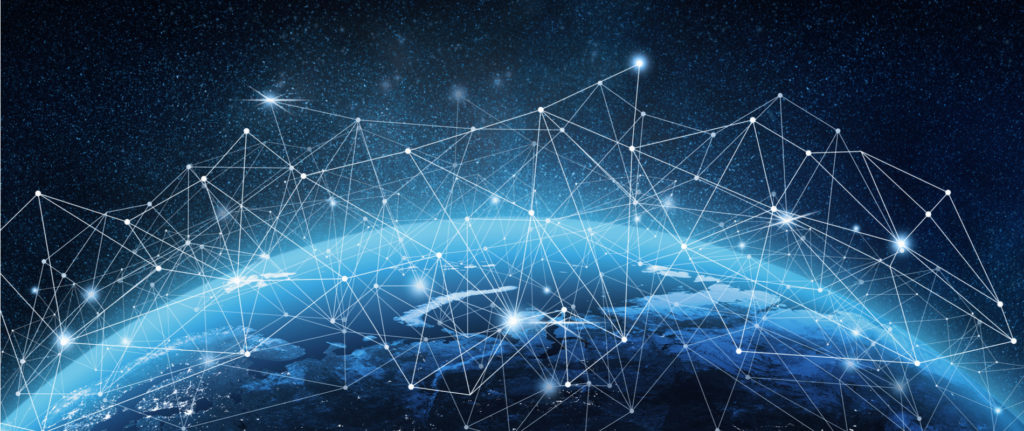
\includegraphics[width=15cm]{redes.jpg}
    \vfill
    \vfill
\end{titlepage}

\newpage
\tableofcontents
\newpage

\section{Introducción a las aplicaciones de red:}
\begin{itemize}

\begin{figure}[h]
\centering
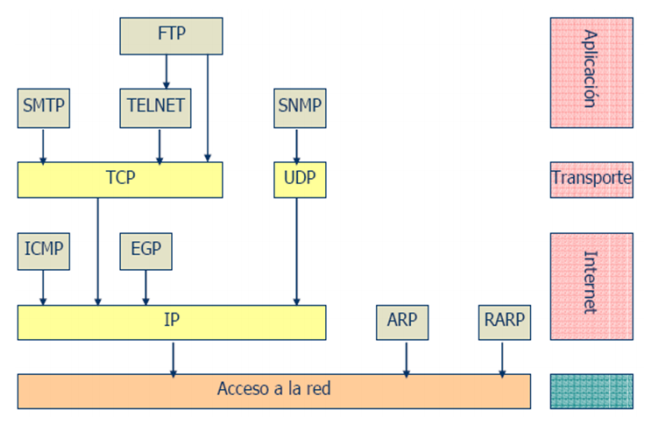
\includegraphics[scale=1,width=1\textwidth]{protocolos.png}
\caption{Esquema Capas}
\end{figure}

\item \textbf{Protocolos de aplicación.}

	\begin{itemize}
		\item \textbf{FTP File Tranfer Protocol:} es un protocolo de red para la transferencia de archivos entre sistemas conectados a una red TCP (CAPA DE TRANSPORTE), basado en la arquitectura cliente-servidor. Este es ofrecido por la capa de aplicación utilizando normalmente los puertos de red 20 y 21 (ver /etc/services). Un problema básico de FTP es que está pensado para ofrecer la máxima velocidad en la conexión, pero no la máxima seguridad, ya que todo el intercambio de información, desde el login y password del usuario en el servidor hasta la transferencia de cualquier archivo, ser realiza en texto plano sin ningún tipo de cifrado, con lo que un posible atacante puede capturar este tráfico, acceder al servidor y/o apropiarse de los archivos transferidos.
		
		\item \textbf{Telnet (Teletype Network):} nombre de un protocolo de aplicación que nos permite acceder a otra máquina para manejarla remotamente como si estuviéramos sentados delante de ella. Para que la conexión funcione, como todos los servicios de internet, la máquina a la que se acceda debe tener un programa especial que reciba y gestione las conexiones. Generalmente se utiliza el puerto 23. También se conecta a una red TCP en la capa de transporte.
		
		\item \textbf{SMTP (Simple Mail Transfer Protocol):} protocolo de aplicación utilizado para el intercambio de mensajes de correo electrónico entre computadoras u otros dispositivos. El funcionamiento de este protocolo se da en línea, de manera que opera en los servicios de correo electrónico. Sin embargo, este protocolo posee algunas limitaciones en cuanto a la recepción de mensajes en el servidor de destino. Como alternativa a esta limitación se asocia normalmente este protocolo con otros, como el POP o IMAP, otorgando a SMTP la tarea específica de enviar correo, y recibirlos empleando los protocolos antes mencionados. Generalmente este protocolo utiliza el puerto 25.
		
		\item \textbf{SNMP (Simple Network Management Protocol):} protocolo de la capa de aplicación que facilita el intercambio de información de administracion entre dispositivos de red (routers, switches, servidores, etc,) Permite a los administradores supervisar el funcionamiento de la red, buscar y resolver sus problemas, y planear su crecimiento. SNMP es un componente de la suite de protocolo de Internet como se define por el IETF. Se compone de un conjunto de normas para la gestión de red, incluyendo una capa de aplicación del protocolo, una base de datos de esquema, y un conjunto de objetos de datos. Generalmente este utiliza el puerto 161. En la capa de transporte este protocolo puede trabajar tanto con UDP como con TCP.
	\end{itemize}
	
\item \textbf{Protocolos de transporte:}
	
	\begin{itemize}
		\item \textbf{TCP (Transmission Control Protocol):} es uno de los protocolos fundamentales de internet. Muchos programas dentro de una red de datos compuesta por redes computadoras, pueden usar TCP para crear 'conexiones' entre sí a través de las cuales puede enviarse un flujo de datos. El protocolo garantiza que los datos serán entregado sin errores y en el orden en que se transmitieron. También proporciona un mecanismo para distinguir aplicaciones dentro de una misma máquina, a través del concepto de puerto. Da soporte a protocolos de aplicación como HTTP, SMTP, SSH y FTP.
		
		\item \textbf{UDP (User Datagram Protocol):} es un protocolo de nivel de transporte basado en el intercambio de datagramas. Permite el envío de datagramas a través de la red sin que se haya establecido previamente una conexión, ya que el propio datagrama incorpora suficiente información de direcciónamiento en su cabecera. Tampoco tiene confirmación de flujo, por lo que los paquetes pueden adelantarse unos a otros; y tampoco se sabe si ha llegado correctamente, ya que no hay confirmación de entrega o recepción. Su uso principal es para protocolos como DHCP, BOOTP, DNS,...
	\end{itemize}

\item \textbf{Protocolos de Internet:}

	\begin{itemize}
		\item \textbf{ICMP Internet Control Message Protocol:} es parte del conjunto de protocolos IP. Es utilizado para enviar mensajes de error e información operativa. Estos mensajes del protocolo ICMP se envían a la dirección IP del origen del paquete. Siendo un protocolo de la 'Capa de Red' ICMP difiere de los protocolos de la 'Capa de Transporte', en que no es en general usado para intercambiar información entre sistemas, ni tampoco por las aplicaciones de usuario (con excepción de algunas herramientas como ping y traceroute, que emplean mensajes ICMP con fines de diagnostico). 
		
		\item \textbf{EGP Exterior Gateway Protocol:} es un protocolo estándar usado para intercambiar información de encaminamiento entre sistemas autónomos. Las puertas de enlace o pasarelas EGP solamente pueden retransmitir información de accesibilidad para las redes de su sistema autónomo. La pasarela debe recoger esta información, habitualmente por medio de un Interior Gateway Protocol(IGP), usado para intercambiar información entre pasarelas del mismo sistema autónomo.
		
		\item \textbf{IP Internet Protocol:} es un protocolo de comunicación de datos digitales clasificado funcionalmente en la capa de red. Su función principal es el uso bidireccional en origen o destino de comunicación para transmitir datos mediante un protocolo no orientado a conexión que transfiere paquetes conmutados a través de distintas redes físicas previamente enlazadas según la norma OSI de enlace de datos.
		
		\item \textbf{ARP Address Resolution Protocol:} es un protocolo de comunicaciones de la capa de enlace, responsable de encontrar la dirección de hardware (MAC) que corresponde a una determinada IP. Para ello se envía un ARP request a la dirección de difusión de la red que contiene la dirección IP por la que se pregunta, y se espera a que esa máquina (u otra) responda (ARP reply) con la dirección Ethernet que corresponade.
		
		\item \textbf{RARP Reverse Address Resolution Protocol:} es un protocolo de comunicaciones utilizado para resolver la dirección IP de una dirección hardware dada. 
	\end{itemize}
\end{itemize}

\textbf{Interacción Cliente/Servidor:} 

La red cliente-servidor es una red de comunicaciones en la cual los clientes están conectados a un servidor, en el que se centralizan los diversos recursos y aplicaciones con que se cuentan; y que los pone a disposición de los clientes una vez que estos son solicitados. Esto significa que todas las gestiones que se realizan se concentran en el servidor, de manera que en él se disponen los requerimientos provenientes de los clientes que tienen prioridad, los archivos que son de uso público y los que son de uso restringido, etc. Características:

\begin{itemize}
\item Servidor:

	\begin{itemize}
		\item Se encuentra siempre en funcionamiento (en background).
		\item Tienen IP permanente y pública.
		\item Los servidores se agrupan en granjas (vease los Data Center de Google)
	\end{itemize}
	
\item Clientes:

	\begin{itemize}
		\item Funcionan intermitentemente.
		\item Su IP puede ser dinámica y privada.
		\item Se comunican con el servidor.
		\item No se comunican con otros clientes.
	\end{itemize}
\end{itemize}

\textbf{Intefaz Socket (Interfaz SOCKS):} es una interfaz (o servicio) de la capa de transporte. La filosofía de la división por capas de un sistema es encapsular, dentro de cada una de ellas, detalles que conciernen sólo a cada capa, y presentársela al usuario de tal forma que este pueda trabajar con ella sin necesidad de conocer sus detalles de implementación. La interfaz de acceso a la capa de transporte del sistema UNIX de Berkeley no está totalmente aislada de las capas inferiores, por lo que a la hora de trabajar con sockets, es necesario conocer algunos detalles sobre esas capas. En concreto, a la hora de establecer una conexión mediante sockets, es necesario conocer la familia o dominio de la conexión y el tipo de conexión. \\

Definimos \textbf{SOCKET} como un descriptor de una transmisión a través del cual la aplicación puede enviar y/o recibir información y/o desde otro proceso de aplicación. Podríamos usar la metáfora de que el SOCKET es una puerta entre aplicación y servicios de transporte.

En la práctica un socket es una variable de tipo puntero a una estructura con los siguientes atributos:

\begin{itemize}
\item Familia (PF\_INET, PF\_UNIX, PF\_APPLETALK,\ldots)
\item Servicio (SOCK\_STREAM = TCP, SOCK\_DGRAM=UDP, SOCK\_RAW=IP o inferiores,\ldots)
\item IP local:
\item IP remota
\item Puerto local
\item Puerto remoto
\end{itemize}

\begin{figure}[h]
\centering
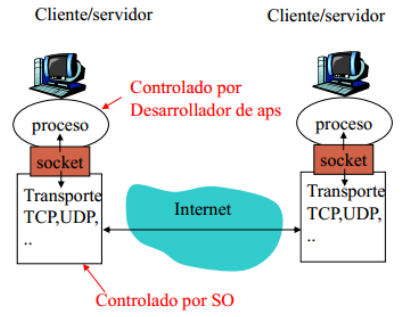
\includegraphics[scale=1,width=0.8\textwidth]{sockets.png}
\caption{Funcionamiento Socket}
\end{figure}

\textbf{Retardo en cola:} Para estimar los retardos (tiempos) en cola se usa la teoría de colas, el uso de un servidor se modela con un sistema M/M/1 (ver glosario). El retardo de cola es:

\begin{equation*}
	R=\frac{\lambda \cdot (T_s)^2}{1-\lambda \cdot T_s}
\end{equation*}

, donde $T_s$ (distribución exponencial) es el tiempo de servicio y $\lambda$ (Poisson) el ratio de llegada de solicitudes. Esta misma expresión se puee utilizar para calcular el retardo en cola en un router. \\

\textbf{Protocolo de aplicación:} un protocolo de la capa de aplicación define cómo los procesos de una aplicación, que se ejecutan en distintos sistemas terminales, se pasan los mensajes entre sí. Para ello el protocolo de aplicación debe definir:

\begin{itemize}
\item El tipo de servicio
	\begin{itemize}
		\item Orientado a conexión o no orientado a conexión.
		\item Realimentado o no realimentado.
	\end{itemize}
\item El tipo de mensaje (request, reponse, $\ldots$).
\item La sintaxis: definición y estructura de 'campos' en el mensaje. En aplicación generalmente son orientados a texto (HTTP), aunque hay excepciones (DNS). La tendencia es usar formato Type-Length-Value.
\item La semántica, es decir, el significado de los campos.
\item Las reglas, cuando los procesos envían mensajes/responden mensajes.
\end{itemize}

Además dentro de los protocolos de aplicación tenemos distintos tipos de protocolos:
\begin{itemize}
\item Protocolos de dominio público: aquellos definidos en los RFC, como por ejemplo HTTP y SMTP.
\item Protocolos propietarios: aquellos que son propiedad de empresas privadas.
\item Protocolos in-band: se opera a través de la misma red la cual se está gestionando.
\item Protocolos out-of-band: se utiliza cuando se quiere independizar el tráfico de gestión de la red que se gestiona.
\item Protocolos stateless: trata cada petición como una transacción independiente que no tiene relación con cualquier solicitud anteiror.
\item Protocolos state-full: cuando el cliente manda una petición al servidor entonces este espera algún tipo de respuesta, si no hay respuesta se reenvia la petición.
\item Protocolos persistentes: aquellos que mantienen la conexión abierta entre sucesiones peticiones.
\item Protocolos no-persistentes (sobre servicios SOC): aquellas que abren y cierran la conexión para cada petición.
\end{itemize}

La tendencia es hacer los protocolos flexibles con una cabecera fija y una serie de 'trozos' (obligatorios y opcionales). Estos trozos pueden incluir una cabecera más específica más una serie de datos en forma de parámetros que pueden ser:

\begin{itemize}
\item Parámetros fijos: en orden
\item Parámetros de longitud variable u opcionales
\item Para los parámetros se utiliza Formato TLV
\end{itemize}

\begin{figure}[h]
\centering
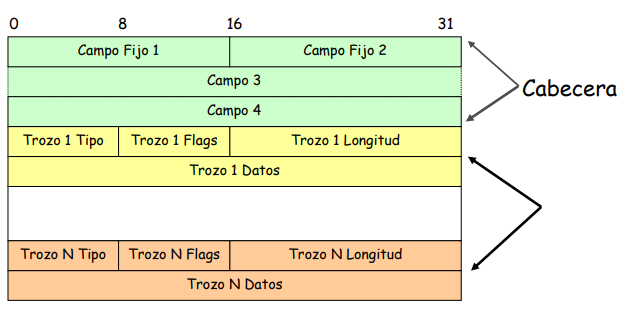
\includegraphics[scale=1,width=1.2\textwidth]{protocolos_aplicacion.png}
\caption{Estructura protocolo de aplicación}
\end{figure}

\begin{figure}[h]
\centering
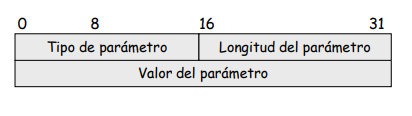
\includegraphics[scale=1,width=0.8\textwidth]{trozo_protocolo.png}
\caption{Estructura de un trozo}
\end{figure}

\textbf{Caracterísiticas/Requisitos de las aplicaciones de red:}
\begin{itemize}
\item \textbf{Tolerancia a pérdidas de datos(errores):} Algunas aplicaiones pueden tolerar algunas pérdidas de datos como el audio y el video. Otras como FTP, telnet, etc, requieren una transferencia 100\% fiable.
\item \textbf{Exigencia de requisitos temporales:} algunas aplicaciones denominadas elásticas requieren retardo (delay) acotado para ser efectivas, otras aplicaciones no.
\item \textbf{Demanda de ancho de banda (tasa de transmisión o throughput):} algunas aplicaciones requieren envío de datos a una tasa determinada, por ejemplo un codec de video, otras no.
\item \textbf{Nivel de seguridad:} los requisitos de seguridad para las distintas aplicaciones son muy variables.
\end{itemize}

En conclusión los requisitos que debe cumplir una aplicación red son muy heterogeneos. \\

\textbf{Protocolos de transporte:} \\

\textbf{Servicios TCP (Transmission Control Protocol):} el modelo de servicio TCP incluye un servicio orientado a conexión y un servicio de transferencia de datos fiable. Cuando una aplicación invoca TCP como su protocolo de transporte, la aplicación recibe ambos servicios de TCP.

\begin{itemize}
\item \textit{Servicio orientado a la conexión.} TCP hace que el cliente y el servidor intercambien entre sí información de control de la capa de transporte \textbf{antes} de que empiecen a fluir los mensajes del nivel de aplicación. Este procedimiento denominado de negociación, de reconocimiento o de establecimiento de la conexión, alerta al cliente y al servidor, permitiéndoles prepararse para el intercambio de paquetes. Después de esta fase de negociación, se dice que existe una conexión TCP entre los sockets de los dos procesos. La conexión es una conexión full-duplex, en el sentido de que los dos procesoso pueden enviarse mensajes entre sí a través de la conexión al mismo tiempo. Una vez que la aplicación ha terminado de enviar mensajes, debe terminar la conexión.

\item \textit{Servicio de transferencia de datos fiable.} Los procesos que se están comunicando pueden confiar en TCP para entregar todos los datos enviados sin errores y en el orden correcto. Cuando un lado de la aplicación pasa un flujo de bytes a un socket, puede contar con TCP para entregar el mismo flujo de bytes al socket receptor sin pérdida ni duplicación de bytes.
\end{itemize}

También incluye un mecanismo de control de congestión, que es un servicio para mejorar el funcionamiento general de internet, más que para el beneficio directo de los procesos que se comunicacn. Este mecanismo de control de congestión regula el proceso emisor (cliente o servidor) cuando la red está congestionada entre el emisor y el receptor.\\

Al igual que incluye un mecanismo de control de congestión, también incluye un mecanismo de control de flujo, que utiliza ventanas deslizantes y se encarga de evitar que un emisor envíe más datos de forma más rápida de la que el receptor puede recibirlos y procesarlos. Se trata de un mecanismo esencial en redes en las que se comunican computadoras con distintas velocidades de transferencia. \\

\textbf{Servicios UDP (User Datagram Protocol):} UDP es un protocolo de transporte ligero y simple que proporciona unos servicios mínimos. No está orientado a conexión, por lo que no tiene lugar un procedimiento de negociación antes de que los dos procesos comiencen a comunicarse. UDP proporciona un servicio de transferencia de datos no fiable; es decir, cuando un proceso envía un mensaje a un socket UDP, el protocolo UDP no ofrece ninguna garantía de que el mensaje vaya a llegar al proceso receptor. Además, los mensajes que sí llegan al proceso receptor pueden hacerlo de manera desordenada. 

UDP no incluye tampoco un mecanismo de control de congestión, por lo que el lado emisor de UDP puede introducir datos en la capa inferior (la capa de red) a la velocidad que le parezca. (Sin embargo, tenga en cuenta que la tasa de transferencia extremo a extremo real puede ser menor que esta velocidad, a causa de la capacidad de transmisión limitada de los enlaces intervinientes o a causa de la congestión). \\

Se usa principalmente en protocolos en los que el intercambio de paquetes de la conexión son mayores o no rentables con respecto a la información transmitida, así como para transmisión de vídeo y audio en tiempo real. \\

TCP y UDP (protocolos de la capa de transporte) al ser usuarios del protocolo IP (protocolo de capa de red) no garantizan Calidad de Servicio (QoS), es decir:

\begin{itemize}
\item El retardo no está acotado.
\item Las fluctuaciones en el retardo no están acotadas.
\item No hay una velocidad de transmisión mínima garantizada
\item No hay una probabilidad de pérdidas acotadas
\end{itemize}

\section{Servicio de Nombres de Dominio (DNS)}
\textbf{DNS Domain Name System:} La comunicación en internet precisa de direcciones IP. Los usuarios normalmente prefieren usar nombres de dominio. El protocolo DNS se encarga de traducir estos nombres a direcciones IP. El Sistema de nombres de dominio (DNS) es una base de datos distribuida implementada en una jerarquía de servidores DNS y un protocolo de la capa de aplicación que permite a los hosts consultar la base de datos distribuida. El protocolo DNS se ejecuta sobre UDP y utiliza el puerto 53.\\

La traducción de nombres de host en direcciones IP se hace del siguiente modo:

\begin{enumerate}
\item La propia máquina cliente ejecuta el lado del cliente de la aplicación DNS.
\item El navegador extrae el nombre de host y pasa el nombre de host al lado del cliente de la aplicación DNS.
\item El cliente DNS envía una consulta que contiene el nombre de host a un servidor DNS.
\item El cliente DNS recibe finalmente una respuesta, que incluye la dirección IP correspondiente al nombre del host.
\item Una vez que el navegador recibe la dirección IP del servidor DNS, puede iniciar una conexión.
\end{enumerate}

De aquí se puede observar que DNS añade un retardo adicional, en ocasiones, sustancial, a las aplicaciones de Internet que le utilizan. DNS proporciona algunos otros servicios importantes además de la traducción de los nombres de host en direcciones IP: 

\begin{itemize}
\item \textbf{Alias de host.} Un host con un nombre complicado puede tener uno o más alias. Por ejemplo, un nombre de host como $relay1.west-coast.enterprise.com$ podría tener, digamos, dos alias como $enterprise.com$ y $www.enterprise.com$. En este caso, el nombre de host $relay1.west-coast.enterprise.com$ se dice que es el nombre de host canónico. Los alias de nombres de host, cuando existe, normalmente son más mnemónicos que los nombres canónicos. Una aplicación puede invocar DNS para obtener el nombre de host canónico para un determinado alias, así como la dirección IP del host.

\item \textbf{Alias del servidor de correo.} Por razones obvias, es enormemente deseable que las direcciones de correo electrónico sean mnemónicas. Una aplicación de correo puede invocar al servicio DNS para obtener el nombre de host canónico para un determinado alias, así como la dirección IP del hsot. De hecho, el registro MX permite al servidor de correo y al servidor web de una empresa tener nombres de host (con alias) iguales; por ejemplo, tanto el servidor web como el servidor de correo de uan empresa se pueden llamar $enterprise.com$.

\item \textbf{Distribución de carga.} DNS también se emplea para realizar la distribución de carga entre servidores replicados, como los servidores web replicados. Los sitios con una gran carga de trabajo, están replicados en varios servidores, ejecutándose cada servidor en un sistema terminal distinto y teniendo cada uno una dirección IP diferente. Para los servidores web replicados hay asociado un conjunto de direcciones IP con un único nombre de host canónico. La base de datos DNS contiene este conjunto de direcciones IP. Cuando los clientes realizan una consulta DNS sobre un nombre asignado a un conjunto de direcciones, el servidor responde con el conuunto completo de direcciones IP, pero rota el orden de las direcciones en cada respuesta. Dado que normalmente un cliente envía su mensajes de solicitud HTPP a la dirección IP que aparece en primer lugar dentro del conjunto, la rotación DNS distribuye el tráfico entre los servidores replicados. La rotación DNS también se emplea para el correo electrónico de modo que múltiples servidores de correo pueden tener el mismo alias. Además, las empresas de distribución de contenido como Akamai han utilizado DNS de formas muy sofisticadas para proporcionar la distribución de contenido web.
\end{itemize}

Estructura jerárquica en dominos: Parte\_local.dominio\_niveln.\ldots.dominio\_nivel1.. Al dominio de nivel 1 se le denomina dominio genérico (.com, .es, .edu, etc.). El domino raíz o '.' está gestionado por ICANN y delega la gestión de algunos dominios genéricos a centros regionales. \\

Inicialmente fueron definidos en RFC 1591 nueve dominos genéricos:

\begin{itemize}
\item .com $\rightarrow$ organizaciones comerciales.
\item .edu $\rightarrow$ instituciones educativas de EEUU
\item .gov $\rightarrow$ instituciones gubernamentales estadounidenses
\item .mil $\rightarrow$ grupos militares de estados unidos
\item .net $\rightarrow$ proveedores de Internet
\item .org $\rightarrow$ organizaciones diversas diferentes de las anteriores
\item .arpa $\rightarrow$ propósitos exclusivos de infraestructura de Internet
\item .int $\rightarrow$ organizaciones establecidas por tratados internacionales entre gobiernos
\item .xy $\rightarrow$ indicativos de la zona geográfica (es: España, jp:Japón).
\end{itemize}

El Sistema de nombres de dominio (DNS) es una base de datos distribuida implementada en una jerarquía de servidores DNS y un protocolo de la capa de aplicación que permite a los hosts consultar la base de datos distribuida, que almacena información asociada a nombres de dominio en redes como internet, con una gestión distribuida. El protocolo DNS se ejecuta sobre UDP y utiliza el puerto 53. \\

\textbf{Una base de datos jerárquica y distribuida}
DNS utiliza un gran número de servidores, organizados de forma jerárquica y distribuidos alrededor de todo el mundo. Ningún servidor DNS dispone de todas las correspondencias de todos los hosts de Internet. En su lugar las correspondencias están repartidas por los servidores DNS.3 niveles de servidores:

\begin{itemize}
\item Servidores raíz '.'. Existen unos 400 servidores reaíz distribuidos por todo el mundo. Trece organizaciones diferentes gestionan estos servidores de nombre de raíz. Los servidores de nombres de raíz proporcionan las direcciones IP de los servidores TLD.

\item Servidores de dominio (Top-Level domain o TLD). Para todos los dominios de nivel superior, como son com, org, net, edu y gov, y todos los dominos de nivel superior correspondientes a los distintos países, como por ejemplo, uk, fr, ca y jp, existe un servidor TLD (o una agrupación de servidores). Los servidores TLD proporcionan las direcciones IP para los servidores DNS autoritativos.

\item Servidores locales o Servidores Autoritativos. Todas las organizaciones que tienen hosts accesibles públicamente (como son los servidores web y los servidores de correo) a través de Internet deben proporcionar registros DNS accesibles públicamente que establezcan la correspondencia entre los nombres de dichos hosts y sus direcciones IP. Un servidor DNS autoritativo de una organización alberga estos registros DNS. Una organización puede elegir implementar su propio servidor DNS autoritativo para almacenar estos registros; alternativamente, la organización puede pagar por tener esos registros almacenados en un servidor NDS autoritativo de algún proveedor de servicios. La mayoría de las universidades y de las empresas de gran tamaño implementan y mantienen sus propios servidores DNS autoritativos principal y secundario (backup).
\end{itemize}

Existe otro tipo importante de servidor DNS conocido como \textbf{servidor DNS local}. Un servidor DNS local no pertenece estrictamente a la jerarquía de servidores, pero no obstante es importante dentro de la arquitectura DNS. Cada ISP (por ejemplo un ISP residencial) tiene un servidor DNS local (también denominado servidor de nombres predeterminado). Cuando un host se conecta a un ISP, este proporciona al host las direcciones IP de uno o más de sus servidores DNS locales (normalmente a través de DHCP). \\

La resolución de nombre de domino puede ser iterativa o recursiva. Para mejorar prestaciones se usan caches. La caché de la DNS es básicamente un registro de los nombres de domino y sus IP asociadas que ya hemos visitado. \\

La base de datos distribuida está formada por un conjunto de servidores cooperativos que almacenan parcialmente la base de datos que se denomina BIND (Berkeley Internet Name Domain). Cada servidor es responsable de una zona, siendo una zona un conjunto de nombres de domino antiguos (por debajo de un nodo en el árbol) de los que un servidor tiene toda la información y es su autoridad. Los servidores autoridad (Start of Authority Servers, es un registro) deben contener toda (no 'cacheada') la información de su zona. La autoridad puede delegarse jerárquicamente a otros servidores. \\

\textbf{Gestión de la base de datos DNS:} 
Los servidores DNS que implementan conjuntamente la base de datos distribuida DNS almacenan los registros de recursos (RR), incluyendo los que proporcionan las correspondencias entre nombre de host y dirección IP. Cada mensaje de respuesta DNS transporta uno o más registros de recursos.

\begin{itemize}
\item Cada zona debe tener al menos un servidor de autoridad:
\item En cada zona hay servidores primarios (almacenan una copia máster de la database en disco locales) y servidores secundarios (obtienen la database por transferencia).
\item La topología real de servidores es complicada: existe 13 servidores raíz (A-M).
\item El root-server F (y otros) tiene un servidor en Madrid (Espanix: punto neutro).
\item Cuando un cliente (a través de un resolver local) solicita una resolución de nombres a su servidor pues ocurrir:
	\begin{itemize}
		\item Respuesta con autoridad: el servidor tiene autoridad en la zona en la que se encuentra el nombre solicitado y devuelve la IP.
		\item Respuesta sin autoridad: el servidor no tiene autoridad sobre la zona en la que se encuentra el nombre solicitado, pero lo tiene en la caché.
		\item No conoce la respuesta: el servidor preguntará a otros servidores de forma recursiva o iterativa. Normalmente se 'eleva' la petición a uno de los servidores raíz.
	\end{itemize}
\end{itemize}

Todo dominio está asociado al menos a un registro Resource Record. Cada RR es una tupla que tiene 5 campos:

\begin{itemize}
\item \textbf{Nombre del dominio:} nombre del dominio al que se refiere el RR.
\item \textbf{Tiempo de vida:} tiempo de validez de un registro (para la caché).
\item \textbf{Clase:} en Internet siempre es IN.
\item \textbf{Tipo de registro:}
	\begin{itemize}
		\item SOA $\rightarrow$ Registro (Start of Authority) con la autoridad de la zona.
		\item NS $\rightarrow$ Registro que contiene un servidor de nombres.
		\item A $\rightarrow$ Registro que define una dirección IPv4.
		\item MX $\rightarrow$ Registro que define un servidor de correo electronico
		\item CNAME $\rightarrow$ Registro que define el nombre canónico de un nombre de dominio
		\item HINFO $\rightarrow$ Información del tipo de máquina y Sistema Operativo.
		\item TXT $\rightarrow$ Información del dominio.
	\end{itemize}
\item \textbf{Valor:} Contenido que depende del campo tipo.
\end{itemize}

\textbf{Mensajes DNS.} Únicamente existen dos calses de mensaje DNS, los mensajes de respuesta y los mensajes de consulta, y ambos utilizan el mismo formato. La semántica en los distintos campos de un mensaje DNS es la siguiente:

\begin{itemize}
\item Los primero 12 bytes constituyen la sección de cabecera, la cual contiene una serie de campos. El primero de estos campos es un número de 16 bits que identifica la consulta. Este identificador se copia en el mensaje de respuesta a la consulta, lo que permite al cliente establecer las corrspondencias correctas entre las respuestas recibidas y las consultas enviadas. En el campo Indicadores se incluyen una serie de indicadores. Un indicador consulta/respuesta de 1bit informa de si el mensaje es una consulta (0) o una respuesta (1). Un indicador autoritativo de 1 bit se activa en un mensaje de respuesta cuando un servidro DNS es un servidor autoritativo para un nombre solicitado. El indicador recursión-deseada, también de 1 bit, se activa cuando el cliente (host o servidor DNS) desea que el servidor DNS realice una recursión cuando no disponga del registro. En un mensaje de respuesta, el campo de recursión-disponible de 1 bit se activa si el servidor DNS soporta la recursión. En la cabecera también se incluyen cuatro campos 'número de', que indican el número de apariciones de los cuatro tipos de secciones de datos que siguen a la cabecera.

\item La sección de cuestiones contiene información acerca de la consulta que se va a realizar. Esta sección incluye un campo de nombre que contiene el nombre que se va a consultar y un campo de tipo que especifica el tipo de cuestión que se plantea acerca del nombre; por ejmplo, la dirección del host asociada con un nombre (tipo A) o el servidor correo para un nomber (tipo MX).

\item En una respuesta de un servidor DNS, la sección respuestas contiene los registros del recurso para el nombre que fue consultado originalmente. Recuerde que en cada registro de recurso existe un parámetro Tipo, un parámetro valor y el parámetro TTL. Una respuesta puede devolver varios registros de recursos, ya que un nombre de host puede tener asociadas varias direcciones IP.

\item La sección autoridad contiene registros de otros servidores autoritativos.

\item La sección información adicional contiene otros registros útiles. Por ejemplo, el campo de respuesta de un mensaje de respuesta a una consulta MX contiene un registro de recurso que proporciona el nombre de host canónico de un servidor de correo. Esta sección de información adicional contiene un registro de tipo A que proporciona la dirección IP para el nombre de host canónico del servidor de correo.
\end{itemize}

\begin{figure}[h]
\centering
\caption{Formato de los mensajes DNS}
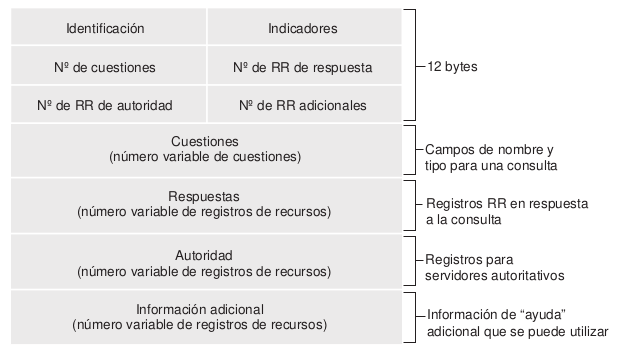
\includegraphics[scale=1,width=1\textwidth]{formato_dns.png}
\end{figure}

Existe una base de datos de resolución inversa para traducir direcciones IP en nombres de dominio. Formato mensajes DNS:
\begin{itemize}
\item DNS se ofrece en el puerto 53 mediante UDP normalmente o TCP (para respuestas grandes $>$ 512 bytes).
\end{itemize}

\section{La navegación web}
El corazón de la Web lo forma el Protocolo de transferecias de hipertexto (HTTP, \textit{HyperText Transfer Protocol}), que es el protocolo de la capa de aplicación de la Web. HTTP se implemente mediante dos programas: un cliente y un servidor. Ambos programas, que se ejecutan en sistemas terminales diferentes, se comunican entre sí intercambiando mensajes HTTP. HTTP define la estructura de los mensajes y cómo el cliente y el servidor intercambian los mensajes. \\

Una página Web (también denominada documento web) consta de objetos. Un objeto es simplemente un archivo (como por ejemplo un archivo HTML, una imagen JPEG, un applet Java o un clip de vídeo) que puede direccionarse mediante un único URL. La mayoría de las páginas web están constituaidas por un archivo base HTML y varios objetos referenciados. Puesto que los navegadores web implementan el lado del cliente HTTP, en el contexto de la Web utilizaremos los términos navegador y cliente indistintamente. Los servidores web, que implementan el lado del servidor HTTP, albergan los objetos web, siendo cada uno de ellos direccionable mediante una URL. \\

esquema:[//[user[:password]@]dominio[:puerto]

[/path][/recurso][?solicitud][\#fragment] 

\begin{figure}[h]
\centering
\caption{Tabla con ejemplos de URL}
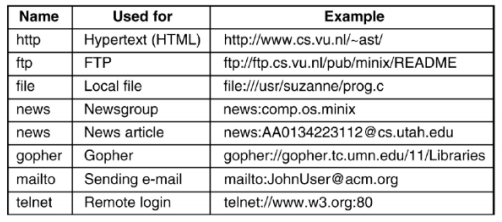
\includegraphics[scale=1,width=1\textwidth]{tabla_navegacion_web.png}
\end{figure}

Las páginas se sirven con el protocolo HTTP: Hyper Text Transfer Protocol. Se trata de un modelo cliente servidor donde el cliente es un browser que solicita, recibe y muestra objetos web, y el servidor envía objetos web en respuesta a peticiones. HTTP utiliza TCP como su protocolo de transporte subyacente. Las páginas web pueden ser estáticas (contenido invariable) o dinámicas (con contenido variable). Las páginas dinámicas pueden proporcionar contenido variables de las siguientes maneras:

\begin{itemize}
\item Usando lenguajes de scripting en el cliente: JavaScript o Flash etc.
\item Usando lenguajes de scripting en el servidor: Perl, PHP, Ruby, Python, etc. Se utilizan incrustando etiquetas dentro de la página web. Cuando el cliente solicita esa web, el servidor web interpreta estas etiquetas para realizar acciones en el servidor generando contenido dinámico. Por ejemplo, insertando información de una base de datos.
\end{itemize}


\textbf{Características HTTP:}
\begin{itemize}
\item Usa los servicios de TCP(S.O.C) en el puerto 80. Inicio de conexión TCP, envío HTTP, cierre de conexión TCP.

\item HTTP es 'stateless' $\rightarrow$ Cookies. El servidor no mantiene información sobre las peticiones de los clientes (su estado) y así ahorra recursos aunque hace más compleja la interacción.

\item Existen dos tipos de servidores:
	
	\begin{itemize}
		\item No persistente $\rightarrow$ se envia únicamente un objeto en cada conexión TCP.
		\item Persistente $\rightarrow$ pueden enviarse multiples objetos sobre una única conexión TCP entre cliente y servidor.
	\end{itemize}
\end{itemize}

\textbf{Mensajes HTTP:}
\begin{enumerate}
\item El cliente HTTP (navegador) solicita un objeto identificado por su URL. Según la configuración del servidor, si no se especifica nada, por defecto se sirve el fichero index.html.
\item El cliente consulta al resolver de DNS por la dirección IP.
\item DNS contesta 150.214.204.231.
\item El cliente abre una conexión TCP al puerto 80 de 150.214.204.231 (3 bandas).
\item El cliente envía una petición 'GET /pages/.../...' (más otra información adicional: cabeceras, cookies, variables, etc).
\item El servidor responde enviando el fichero 'index.html' por la misma conexión.
\item Al usar TCP el cliente y servidor de HTTP reciben un servicio orientado a conexión, fiable, sin errores, con control de flujo, con control de congestión, etc. Es decir una comunicación TRANSPARENTE y FIABLE.
\item Si es persistente se siguen solicitando objetos de la página por la conexión.
\item Se cierra la conexión TCP y se liberan recursos en el servidor y cliente.
\item El cliente visualiza el contenido.
\end{enumerate}


\textbf{HTTP definde dos tipos de mensajes (request,response):}
\begin{enumerate}
\item HTTP request message (solicitudes del cliente al servidor). La primera línea de un mensaje de solicitud HTTP se denomina \textbf{línea de solicitud} y las siguientes son las \textbf{líneas de cabecera}. La línea de solicitud consta de tres campos: el campo método, el campo URL y el campo de la versión HTTP. El campo que especifica el método puede tomar valores, entre los que se incluyen GET, POST, HEAD, PUT y DELETE. La inmensa mayoría de los mensajes de solicitudad HTTP utilizan el método GET. Este método se emplea cuando el navegador solicita un objeto, identificándose dicho objeto en el campo URL. La linea de cabecera 'Host:' especifica el host en el que reside el objeto. Al incluir la línea de cabecera 'Connection: close', el navegador está diciendo al servidor que no desea molestarse en trabajar con conexiones persistentes, sino que desea que el servidor cierre la conexión después de enviar el objeto solicitado. La línea 'User-agent:' especifica el agente de usuario, es decir, el tipo de navegador que está haciendo la solicitud al servidor. Finalmente la línea 'Accept-Lenguage:' indica que el usuario prefiere recibir una versión en francés del archivo.
	\begin{figure}[h]
		\centering
		\caption{HTTP request message}
		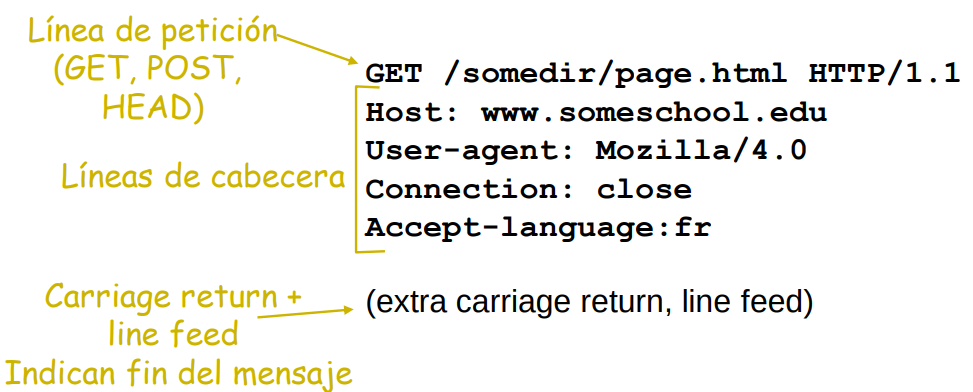
\includegraphics[scale=1,width=0.8\textwidth]{mensaje_request.png}
	\end{figure}
	
\item HTTP response message: (respuestas del servidor al cliente). Los mensajes de respuesta tienen tres secciones, una línea de estado inicial, seis líneas de cabecera y después el cuerpo de entidad. El cuerpo de entidad es la parte más importante del mensaje, ya que contiene el objeto solicitado en sí. La línea de estado contiene tres campos: el que especifica la versión del protocolo, un código de estado y el correspondiente mensaje explicativo. En las líneas de cabecera, la línea 'Connection: close' indica al cliente que el servidor va a cerrar la conexión TCP después de enviar el mensaje. La línea 'Date:' indica hora y fecha a la que se creó la respuesta HTTP y fue enviada por el servidor. La línea 'Server:' indica porque servidor fue creado el mensaje. La línea 'Last-Modified:' resulta fundamental para el almacenamiento en caché del objeto, tanto en el cliente local como en los servidores de almacenamiento caché de la red. La linea 'Content-Length:' especifica el número de bytes del objeto que está siendo enviado. La línea 'Content-Type:' indica que el objeto incluido en el cuerpo de entidad es texto HTML.
	\begin{figure}[h]
		\centering
		\caption{HTTP response message}
		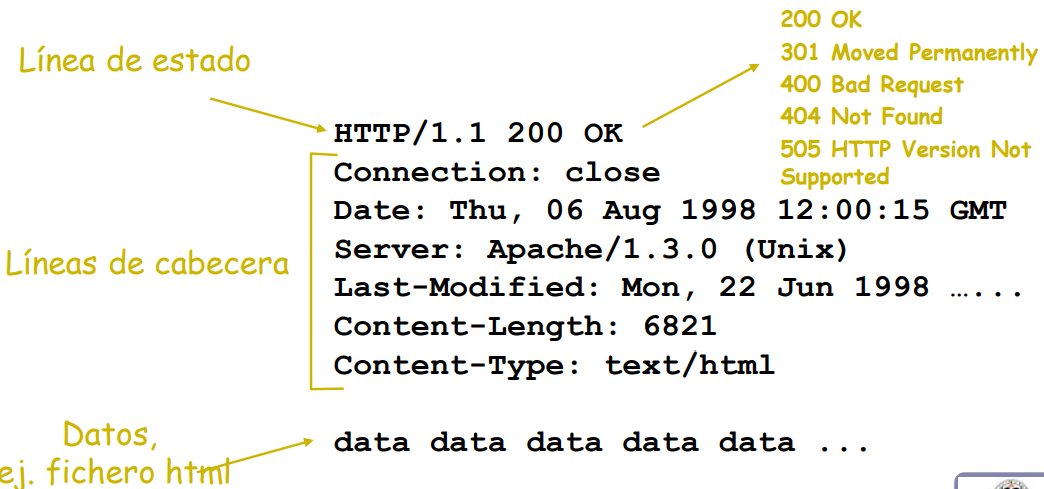
\includegraphics[scale=1,width=0.8\textwidth]{mensaje_respuesta.png}
	\end{figure}
\end{enumerate}

\textbf{PROTOCOLO HTTP 1.1}

\begin{itemize}
\item Métodos (acciones solicitadas por los clientes en los request messages):
	\begin{itemize}
		\item \textbf{OPTIONS:} solicitud de infromación sobre las opciones disponibles.
		\item \textbf{GET:} solicitud de un recurso (puede ser condicional)
		\item \textbf{HEAD:} igual que GET pero el servidor no devuelve el cuerpo sólo cabeceras
		\item \textbf{POST:} solicitud al servidor para que acepte y subordine a la URI especificada, los datos incluidos en la solicitud.
		\item \textbf{PUT:} solicitud de sustituir la URI especificada con los datos incluidos en la solicitud.
		\item \textbf{DELETE:} solicitud de borrar la URI especificada.
	\end{itemize}
	
\item Códigos de respuesta (para los response messages del servidor):
	\begin{itemize}
		\item 1xx indican mensajes exclusivamente informativos. 
		\item 2xx indican algún tipo de exito (200 OK, la solicitud se ha ejecutado con éxito y se ha devuelto la información en el mensaje de respuesta).
		\item 3xx redirección al cliente a otra URL  (301 Moved Permanently, el objeto solicitado ha sido movido de forma permanente; el nuevo URL se especifica en la línea de cabecera 'Location:' del mensaje de respuesta. El software del cliente recuperará automáticamente el nuevo URL).
		\item 4xx un error  (404 Not Found, el documento solicitado no existe en este servidor).
		\item 5xx indican un error (505 HTTP Version Not Supported, la versión de protocolo HTTP solicitada no es soportada por el servidor).
	\end{itemize}
	
\item Cabeceras(47 request headers y 49 response headers): las cabeceras HTTP permiten al cliente y al servidor enviar información adicional junto con una petición o respuesta. Una cabecera de petición está compuesta por su nombre (no sensible a mayúsculas) seguido de dos puntos ':', y a continucación su valor (sin saltos de línea). Los espacios en blanco a la izquierda del valor son ignorados.
	\begin{verbatim}
		From: , User-Agent:, Content-Type:, Content-Length:,...
	\end{verbatim}
\end{itemize}

Dentro de las cabeceras destacamos las siguientes que son comunes para peticiones y respuestas:

\begin{itemize}
\item \textbf{Content-Type:} descripción MIME (Multipurpose Internet Mail Extensions) de la información contenida en este mensaje.

\item \textbf{Content-Lenght:} longitud en bytes de los datos enviados, expresado en base decimal.

\item \textbf{Content-Encoding:} formato de codificación de los datos enviados en este mensaje. Sirve, por ejemplo, para enviar datos comprimidos o encriptados.

\item \textbf{Date:} fecha local de la operacion. Las fechas deben incluir la zona horaria en que reside el sistema que genera la operación. Ej: Sunday, 12-Dec-96 12:21:22 GMT+01. No existe un formato único para las fechas.
\end{itemize}

También se destacan las siguientes cabeceras sólo para peticiones del cliente:

\begin{itemize}
\item \textbf{Accept:} campo opcional que contiene una lista de tipos MIME aceptados por el cliente.

\item \textbf{Authoritation:} clave de acceso que envía un cliente para acceder a un recurso de uso protegido o limitado. La información incluye el formato de autorización empleado, seguido de la clave de acceso propiamente dicha.

\item \textbf{From:} campo opcional que contiene la dirección de correo electrónico del usuario del cliente Web que realiza el acceso.

\item \textbf{If-Modified-Since:} permite realizar operaciones GET condicionales, en función de si la fecha de modificación del objeto requerido es anterior o posterior a la fecha proporcionada. Puede ser utilizada por los sitema de almacenamiento temporal de páginas. Es equivalente a realizar un HEAD seguido de un GET normal.

\item \textbf{Referer:} contiene la URL del documento desde donde se ha activado este enlace. De esta forma, un servidor puede informar al creador de ese documento de cambios o actualizaciones en los enlaces que contiene. No todos los cliente lo envían.

\item \textbf{User-agent:} cadena que identifica el tipo y versión del cliente que realiza la petición. Por ejemplo, los browser de Netscape envían cadenas del tipo User-Agent:Mozilla/3.0(WinNT;I).
\end{itemize}

Destacamos cabeceras sólo para respuestas del servidor HTTP:

\begin{itemize}
\item \textbf{Allow:} informa de los comandos HTTP opcionales que se pueden aplicar sobre el objeto al que se refiere esta respuesta. Por ejemplo, Allow:GET, POST.

\item \textbf{Expires:} fecha de expiración del objeto enviado. Los sitemas de cache deben descartar las posibles copias del objeto pasada esta fecha. Por ejemplo, Expires: Thu, 12 Jan 97 00:00:00 GMT+1. No todos los sitemas lo envían.

\item \textbf{Last-modified:} fecha local de modificación del objeto devuelto. Se puede corresponder con la fecha de modificación de un fichero en disco, o, para información generada dinámicamente desde una base de datos, con la fecha de modificación del registro de datos correspondiente.
\end{itemize}

\textbf{Web Caché:}  una caché web, también denominada servidor proxy, es una entidad de red que satisface solicitudes HTTP en nombre de un servidor origne. Para conseguir esto el usario configura el browser para que el acceso web sea vía caché. La caché web dispone de su propio almacenamiento en disco y mantiene en él copias de los objetos solicitados recientemente. Funcionamiento: 

\begin{enumerate}
\item El navegador establece una conexión TCP con la caché web y envía una solicitud HTTP para el objeto a la caché web.

\item La caché web comprueba si tiene una copia del objeto almacenada localmente. Si la tiene, la caché web devuelve el objeto dentro de un mensaje de respuest HTTP al navegador del cliente.

\item Si la caché web no tiene el objeto, abre una conexión TCP con el servidor de origen. La caché web envía entonces una solicitud HTTP para obtener el objeto a través de la conexión TCP caché-servidor. Después de recibir esta solicitu, el servidor de origen envía el objeto dentro de un mensaje de respuest HTTP a la caché web.

\item Cuando la caché web recibe el objeto, almacena una copia en su dispositivo de almacenamiento local y envía una copia, dentro de un mensaje de respuesta HTTP, al navegador del cliente (a través de la conexión TCP existente entre el navegador del cliente y la caché web).
\end{enumerate}

\begin{figure}[h]
\centering
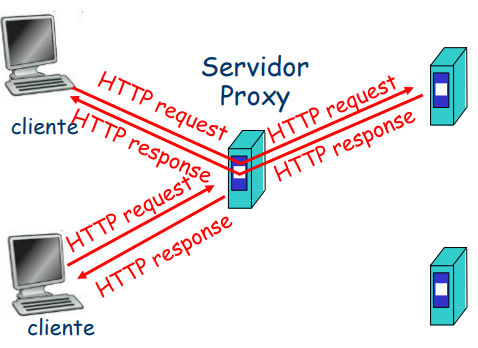
\includegraphics[scale=1,width=0.8\textwidth]{web_cache.png}
\caption{Ejemplo Cliente-Servidor con peticiones HTTP}
\end{figure}

Un ejemplo de respuesta típica de un servidor configurado para gestionar cachés sería:

\begin{verbatim}
HTTP/1.1 200 OK
Date: Fri, 30 Oct 1998 13:19:41 GMT
Server: Apache/1.3.3(Unix)
Cache-Control: max-age=3600
Expires: Fri, 30 Oct 1998 13:19:41 GMT
Last-Modified: Mon, 29 Jun 1998 02:28:12 GMT
ETag: "3e86-410-3596fbbc"
Content-Length: 1040
Content-Type: text/html
\end{verbatim}

Las cabeceras se asocian al fichero en la caché local. También es objetivo de la web caché no enviar objetos si el caché tiene la versión actualizada.

\begin{itemize}
\item \textbf{Cache:} especifica la fecha de la copia en el requerimetno HTTP

\begin{verbatim}
If-modified-since: <date>
If-None-Match:
	"686897696a7c876b7e"
\end{verbatim}

\item \textbf{Servidor:} responde sin el objeto si la copi de la cache es la última.

\begin{verbatim}
HTTP/1.0 304 Not Modified

\end{verbatim}
\end{itemize}

\begin{figure}[h]
\centering
\caption{Diagrama de mensajes cache-servidor}
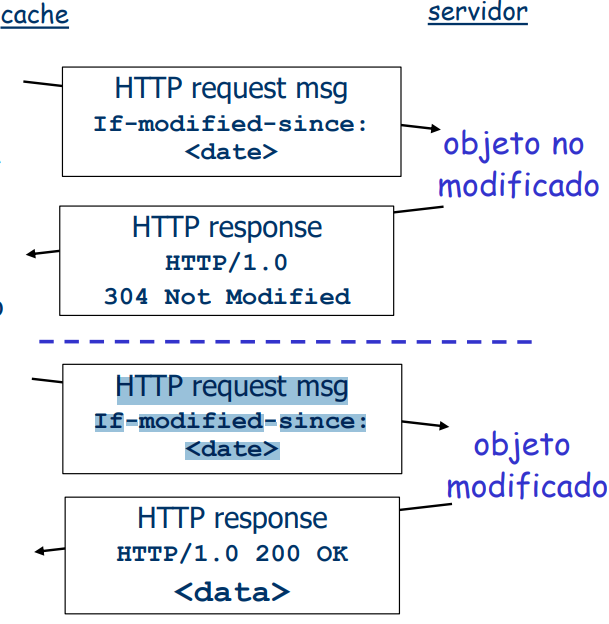
\includegraphics[scale=1,width=0.8\textwidth]{ejemplo_mensajes_web_cache.png}
\end{figure}

\textbf{Cookies.} Se sabe que un servidor HTTP de por si no tiene memoria del estado de la conexión. Sin embargo, para un sitio web, a menudo es deseable poder identificar a los usuarios, y para esto propósitos HTTP utiliza cookies. Las cookies permite a los sitios seguir la pista de los usuarios.  

La tecnología de las cookies utiliza 4 componentes: (1) una línea de cabecera de la cookie en el mensaje de respuesta HTTP; (2) una línea de cabecera en el mensaje de solicitud HTTP;(3) el archivo de cookies almacenado en el sistema terminal del usuario y gestionado por el navegador del usuario;(4) una base de datos back-end en el sitio web. \\

La primera vez que un usuario accede a un determinado documento de un servidor, éste proporciona una cookie que contiene datos que relacionarán posteriores operaciones. El cliente almacena la cookie en su sistema para usarla después. En los futuros accesos a este servidor, el navegador podrá proporcionar la cookie original, que servirá de nexo entre este acceso y los anteriores. Todo este proceso se realiza automáticamente, sin intervención del usuario. \\

Su aplicación más inmediata son los sistemas de compra electrónica. Estos supermercados virtuales necesitan relacionar el contenido pedido con el cliente que lo ha solicitado. Otro uso muy insteresante son los sistemas personalizados de recepción de información, en los que es posible construir una página a medida, con información procedente de fuentes muy diversas. En accesos sucesivos, el cliente enviará la cookie, y el serivdor podrá generar una página personalizada con las preferencias del usuario. \\

Por último, algunas compañías emplean las cookies para realizar un seguimiento de los accesos a sus servidores WWW, identificando las páginas más visitadas, la manera en que se pasa de una a otra sección, etc. \\

Un servidor HTTP envía los diferentes campos de una cookie con la nueva cabecera HTTP Set-Cookie:

\begin{verbatim}
Set-Cookie: 
Domain=www.unican.es;
Path=/;
Nombre=Luis;
Expires Fri, 15-Jul-97 12:00:00 GMT
\end{verbatim}

Cuando se accede a una URL que verifica el par dominio/path registrado, el cliente enviará automaicamente la información de los diferentes campos de la cookie con la nueva cabecera HTTP Cookie:

\begin{figure}[h]
\centering
\caption{Diagrama paso de mensajes con cookies}
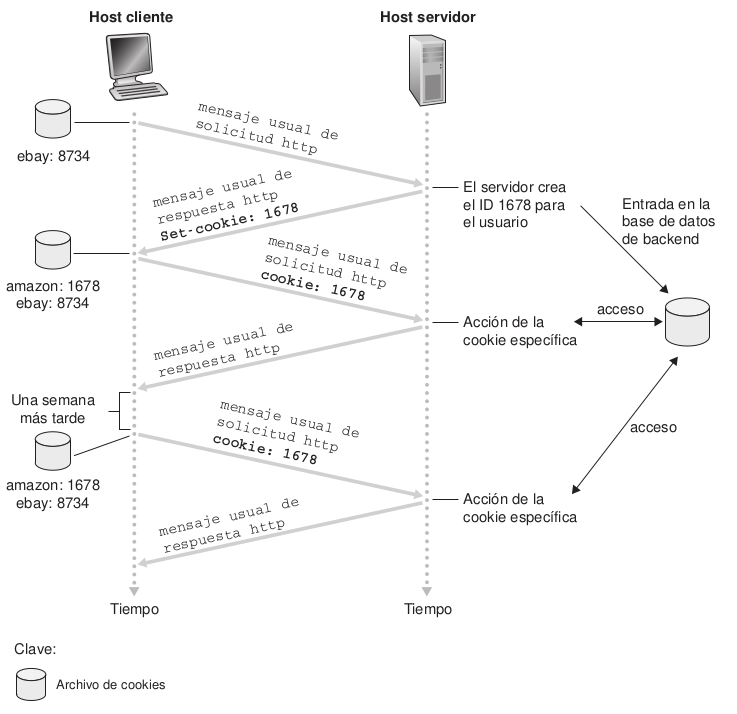
\includegraphics[scale=1,width=0.8\textwidth]{paso_mensajes_cookie.png}
\end{figure}

\textbf{Acceso restringido}

HTTP no es seguro, pero incluye cabeceras \textit{WWW-Authenticate} y \textit{Authorization} para restringir el acceso a recursos. Este es vulnerable a ataques por repetición.

\begin{figure}[h]
\centering
\caption{Diagrama de mensajes Cliente-Servidor con checkeo de credenciales}
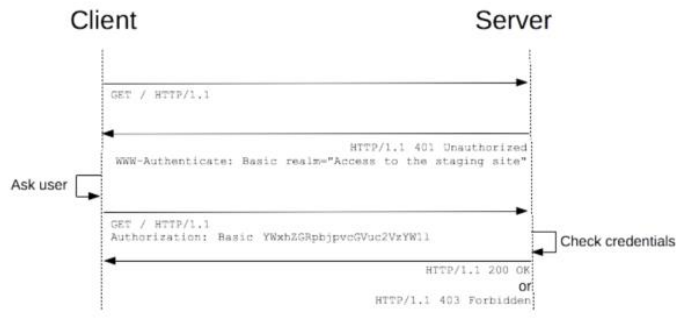
\includegraphics[scale=1,width=1\textwidth]{diagrama_cliente_servidor.png}
\end{figure}

\begin{verbatim}
WWW-Authenticate: <type> realm=<realm>[, charset="UTF-8"]
\end{verbatim}

Donde $WWW-Authenticate$ define el método de autenticación que debería ser usado para tener acceso al contenido. $<type$ indica el tipo de autenticación, $<realm>$ es una descripción del recurso protegido. Si realm no es especificado, los clientes a menudo muestran el hostname. Finalmente $charset$ indica al cliente el tipo de encoding preferido por el servidor cuando se envía un nombre de usuario y contraseña. El único valor permitido es la cadena de texto 'UTF-8'.

\begin{verbatim}
Authorization: <type> <credential>
\end{verbatim}

Por su parte $Authorization$ contiene las credenciales para autenticar a un usuario con un servidor. $<type>$ indica el tipo de autenticación, donde uno de los tipos más comunes es 'Basic'. Por su parte $<credential>$, si $<type>$ es $BASIC$ incluye el $username:password$ codificado en BASE64.

\section{El correo electrónico}
Entre los elementos y protocolos principales del correo electrónico:

\begin{itemize}
\item \textbf{Cliente de correo (\textit{Mail User Agent})}

\item \textbf{Servidor de correo (\textit{Mail Server ó Mail Transfer Agent})}

\item \textbf{Protocolo de envío}: Simple Mail Transfer Protocol (SMTP)

\item \textbf{Protocolos de descarga (o lectura):} POP3, IMAP, HTTP
\end{itemize}

\textbf{Agente de usuario (\textit{Mail User Agent}):} permiten a los usuarios leer, responder, reenviar, guardar y componer mensajes. Por ejemplo, Outlook, Thunderbird, etc. \\

\textbf{Servidor de correo (\textit{Mail Transfer Agent}):} reenvía mensajes salientes y almacena en buzones los mensajes entrantes de cada usuario. \\

Cada destinatario tiene un buzón de correo ubicado en uno e os servidores de correo.

\begin{figure}[h]
\centering
\caption{Ejemplo Diagrama Cliente-Servidor de Correo Electrónico}
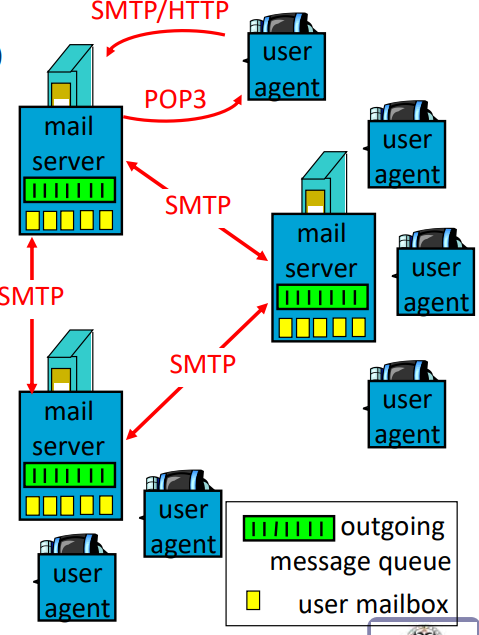
\includegraphics[scale=1,width=0.6\textwidth]{ejemplo_smtp.png}
\end{figure}

SMTP se miplementa mediante dos programas (incluidos ambos en cada mail server):

\begin{itemize}
\item \textbf{Cliente SMTP:} se ejecuta en el mail server (MTA) que está enviando correo.
\item \textbf{Servidor SMTP:} se ejecuta en el mail server (MTA) que está recibiendo correo.
\end{itemize}

\textbf{'sendmail':} es una facilidad de enrutamiento entre redes de propósito general que soporta varios tipos de transfernecias de correo y métodos de entrega, incluyendo SMTP usado para el transporte de email en Internet. \\

SMTP usa TCP en el puerto 25, y es un protocolo orientado a texto. SMTP es un protocolo orientado a conexión, es \textit{in-band} y es \textit{state-full}. Este prtocolo implica tres fase, el \textit{handshaking} o saludo, la transferencia de mensajes y el cierre de la conexión. \\

La interacción entre cliente SMTP y servidor SMTP se realiza mediante comandos y respuestas, donde los comandos están escritos en texto ASCII y las respuestas son códigos de estado y frases explicativas. \\

SMTP restringe el cuerpo (no sólo las cabeceras) de todos los mensajes a formato ASCII de 7 bits, lo cual caus problemas en la actualidad, pues requiere que los datos bianrios multimedia se codifiquen a ASCII antes de ser transmitidos a través de SMTP y requiere que el correspondiente mensaje ACII sea decodificado de vuelta a binario una vez realizado el transporte SMTP. Con la definición posterior de las extensiones MIME se puede enviar ASCII de 8 bits y formatos enriquecidos. \\

En el envío/recepción de un correo se sigue la siguiente secuencia de pasos:

\begin{enumerate}
\item El usuario origen compone mediante su Agente de Usuario (MUA) un mensaje dirigido a la dirección de correo electrónico del usuario destino.

\item Se envía con SMTP (ó HTTP) el mensaje al servidor de correo (MTA) del usuario origen que lo sitúa en la cola de mensajes salientes. 

\item El cliente SMTP abre una conexión TCP con el servidor de correo (MTA) (obtenido por DNS) del usuario destino. 

\item El cliente SMTP envía el mensaje sobre la conexión TCP.

\item El servidor de correo del usuario destino ubica el mensaje en el buzón del usuario destino.

\item El usuario destino invoca a su Agente de Usuario (MUA) para leer el mensaje utilizando POP3, IMAP ó HTTP.
\end{enumerate}

\begin{figure}
\centering
\caption{Esquema de funcionamiento SMTP}
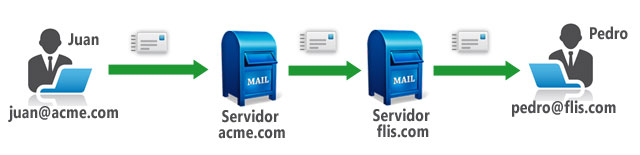
\includegraphics[scale=1,width=1\textwidth]{envio-recepcion.jpg}
\end{figure}

Es importante observar que normalmente SMTP no utiliza servidores de correo intermedios para enviar correo, incluso cuando los dos servidores de correo se encuentran en extremos opuestos del mundo. \\

\begin{figure}[h]
\centering
\caption{Comandos SMTP cliente}
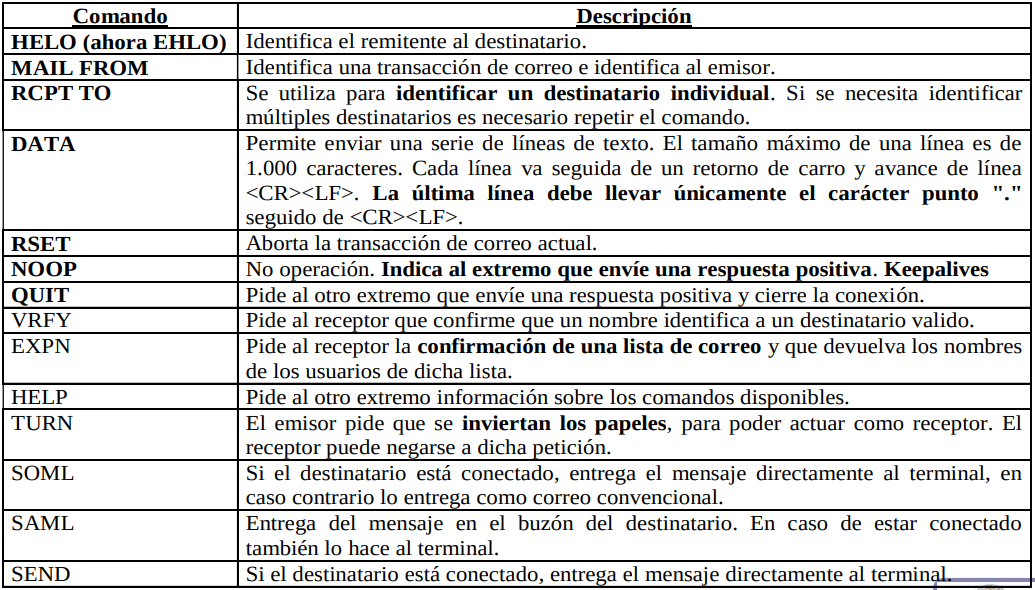
\includegraphics[scale=1,width=1.1\textwidth]{comando_smtp_cliente.png}
\end{figure}

Veamos  en detalle cómo transfiere SMTP un mensaje desde un servidor de correo emisor a un servidor de correo receptor. En primer lugar, el cliente SMTP (que se ejecuta en el host servidor de correo emisor) establece una conexión TCP con el puerto 25 del servidor SMTP (que se ejecuta en el host del servidor de correo receptor).  Si el servidor no está operativo, el cliente lo intentará más tarde. Una vez que se ha establecido la conexión, el servidor y el cliente llevan a cabo el proceso de negociación de la capa de aplicación. Durante esta fase de negociación SMTP, el cliente SMTP especifica la dirección de correo electrónico del emisor y la dirección de correo electrónico del destinatario. Una vez que el cliente y el servidor SMTP se han presentado a sí mismo, el cliente envía el mensaje. SMTP cuenta con el servicio de transferencia de datos fiable de TCP para transferir el mensaje al servidor sin errores. El cliente repite entonces este proceso a través de la misma conexión TCP si tiene que enviar otros mensajes al servidor; en caso contrario, indica a TCP que cierre la conexión. A continuación se muestra un ejemplo de mensajes entre clientes y servidor. Los mensajes que el cliente manda a su socket van precedido por C y los del servidor a su socket por S:

\begin{verbatim}
S: 220 hamburger.edu
C: HELO crepes.fr
S: 250 Hello crepes.fr, pleased to meet you
C: MAIL FROM: <alicia@crepes.fr>
S: 250 alicia@crepes.fr ... Sender ok
C: RCPT TO: <benito@hamburger.edu>
S: 250 bob@hamburger.edu ... Recipient ok
C: DATA
S: 354 Enter mail, end with ”.” on a line by itself
C: ¿Te gusta el ketchup?
C: ¿Y los pepinillos en vinagre?
C: .
S: 250 Message accepted for delivery
C: QUIT
S: 221 hamburger.edu closing connection
\end{verbatim}

\begin{figure}[h]
\centering
\caption{Códigos de respuesta SMTP del servidor}
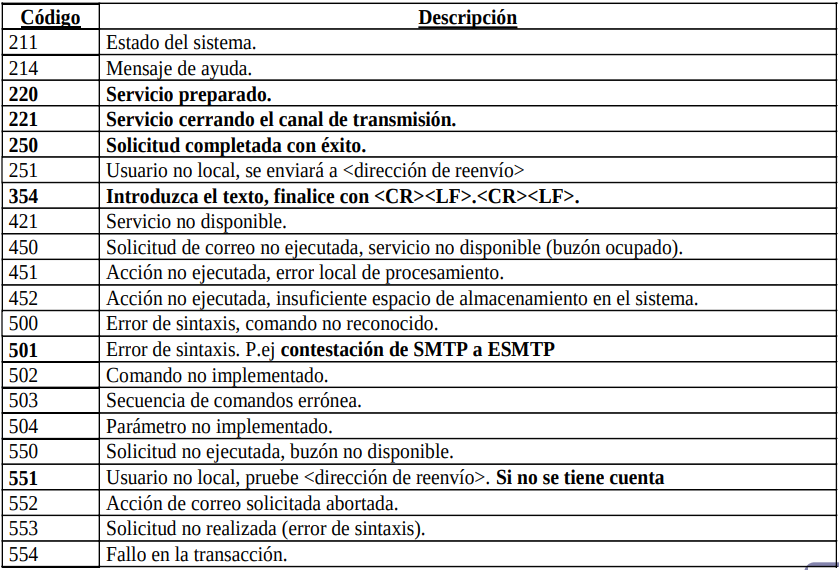
\includegraphics[scale=1,width=1.1\textwidth]{codigo_smtp_servidor.png}
\end{figure}

Toda cabecera de un mail debe estar formada por una línea de cabecera 'From:' y una línea de cabecera 'To:' y también puede incluir una línea de cabecera 'Subject:', así como toras líneas de cabecera opcionales. Es importante destacar que estas líneas de cabecera son diferentes de los comandos SMTP que ya se ahn visto. Los comandos vistos forman parte del protocolo de negociación SMTP; las líneas de cabecera por su parte forman parte del propio mensaje de correo.

\begin{verbatim}
From:alice@crepes.fr
To:bob@hamburger.edu
Subject: Picture of yummy crepe.
MIME-Version: 1.0 ##########Versión MIME
Content-Transfer-Encoding: base64 ##########Método de codificación
Content-Type: image/jpeg ##########Datos multimedia, tipo, subtipo, \ldots

base64 encoded data \ldots
................................ ##########Datos codificados
........... base 64 encoded data
\end{verbatim}

\textbf{MIME (Multipurpose Internet Mail Extensions): Content-Type:tipos y subtipos.} La lista inicial de tipos y subtipos especificados por el RFC 1521 se muestra en la figura 16.

\begin{figure}[h]
\centering
\caption{Tipos y subtipos de MIME:Content-Type}
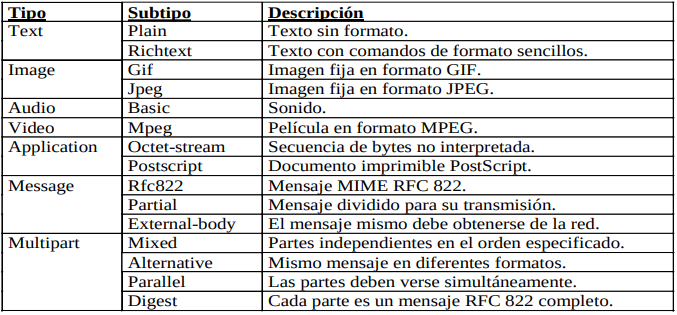
\includegraphics[scale=1,width=1.1\textwidth]{tipos_subtipos_mime.png}
\end{figure}

\textbf{MIME: Content-Type: tipo application:} el tipo application es un tipo general para los formatos que requieren procesamiento externo no cubierto por ninguno de los otros tipos. El subtipo 'octet-stream' simplemente es un secuencia de bytes no interprestados, tal que a su recepción, un agente de usuario debería presentarla en pantalla sugiriendo al usuario que se copie en un archivo y solicitando un nombre de archivo. El subtipo 'postcript', se refiere al lenguaje PostScript de Adobe Systems. Aunque una gente de usuario puede llamar a un intérprete PostScript externo para visualizarlo, hacerlo no está exento de riesgos al ser PostScript un lenguaje de programación incompleto. \\

\textbf{MIME: Content-Type: tipo message:} el tipo 'message' permite que un mensaje esté encapsulado por completo dentro de otro. Este esquema es útil para reenviar correo electrónico. El subtipo 'rfc822' se utiliza cuando se encapsula un mensaje RFC 822 completo en un mensaje exterior. El subtipo 'partial hace posible dividir un mensaje encapsulado en pedazos y enviarlos por separado. Los parámetros hacen posible ensamblar correctamente todas las partes en el destino. El subtipo 'external-body' puede usarse para mensajes muy grande, por ejemplo, películas de vídeo. En lugar de incluir el archivo MPEG en el mensaje, se da una dirección FTP y el agente recepto puede obtenerlo a través de la red cuando se quiera. \\

\textbf{MIME: Content-Type: tipo multipart:} el tipo 'multipart', permite que un mensaje contenga más de una parte, con el comienzo y el fin de cada parte claramente delimitados. El subtipo 'mixed' permite que cada parte sea diferente. El subtipo 'alternative' indica que cada parte contiene el mismo mensaje, pero expresado en un medio o codificación diferente. El subtipo 'parallel' se usa cuando todas las partes deben 'verse' simultáneamente, por ejemplo, en los canales de audio y vídeo de las películas. El subtipo 'digest' se usa cuando se juntan muchos mensajes en un mensaje compuesto. \\

\begin{figure}[h]
\centering
\caption{Ejemplo Multipart/Mixed}
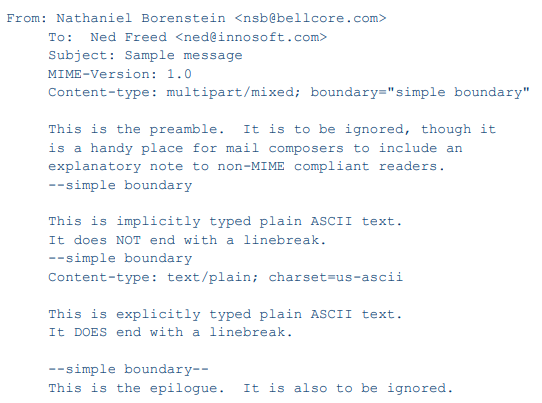
\includegraphics[scale=1,width=0.8\textwidth]{ejemplo_multipart_fixed.png}
\end{figure}

\textbf{Protocolo de acceso POP3 (Post Office Protocol-Version 3):} es un protocolo de acceso a correo extremadamente simple. Dado que el protocolo es tan simple, su funcionalidad es limitada. POP3 se inicia cuando el agente de usuario (el cliente) abre una conexión TCP en el puerto 110 al servidor de correo (el servidor). Una vez establecida la conexión TCP, POP3 pasa a través de 3 fases: autorización, transacción y actualización. Durante la primera fase, la autorización, el agente de usuario envía un nombre de usuario y una contraseña (en texto legible) para autenticar al usuario. Durante la segunda fase, el agente de usuario recupera los mensajes; también durante esta fase, el agente de usuario puede marcar los mensajes para borrado, eliminar las marcas de borrado y obtener estadísiticas de correo. La tercera fase, la actualización, tiene lugar después que el cliente haya ejecutado el comando 'quit', terminando la sesión POP3; en este instante, el servidor de correo borra los mensajes que han sido marcados para borrado. 

En una transacción POP3, el agente de usuario ejecuta comandos y el servidor devuelve para cada comando una respuesta. Existen dos posibles respuestas, OK (seguida en ocasiones por una serie de datos servidor-cliente), utilizada por el servidor para indicar que el comando anterior es correcto; y -ERR, utilizada por el servidor para indicar que había algún error en el comado anterior.

La fase de autorización tiene dos comandos principales: 'user <nombreusuario>' y 'pass <contraseña>'. Para ilustrar esto suponga que mailServer es el nombre de un servidor de correo. Verá algo similar a:

\begin{verbatim}
telnet mailServer 110
+OK POP3 server ready
user benito
+OK
pass hambre
+OK user successfully logged on
\end{verbatim}

\textbf{Comandos POP3:}
\begin{figure}[h]
\centering
\caption{Comandos POP3}
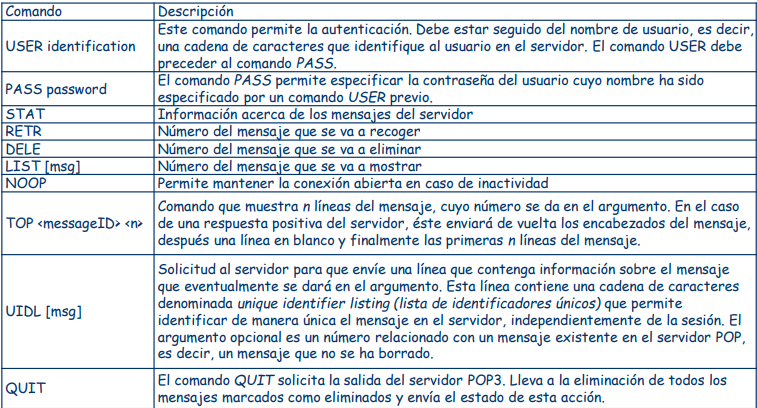
\includegraphics[scale=1,width=1.1\textwidth]{comando_pop3.png}
\end{figure}

Un agente de usuario que utilice POP3 suele ser configurado para 'descargar y borrar' o para 'descargar y guardar'. La secuencia de comandos que ejecute un agente de usuario POP3 dependerá de en cuál de estos dos modos esté operando. En el modo descargar y borrar, el agente de usuario ejecutará los comandos, list, retr y dele. Por ejemplo, suponga que el usuario tiene dos mensajes en su buzón de correo. En el diálogo que proporcionamos a continucación, C (cliente) es el agente de usuario y S (servidor) es el servidor de correo. La transacción sería similar a lo siguiente:

\begin{verbatim}
C: list
S: 1 498
S: 2 912
S: .
C: retr 1
S: (bla bla ...
S: .................
S: ..........bla)
S: .
C: dele 1
C: retr 2
S: (bla bla ...
S: .................
S: ..........bla)
S: .
C: dele 2
C: quit
S: +OK POP3 server signing off
\end{verbatim}

\begin{figure}[h]
\centering
\caption{Ejemplo Protocolo POP3 TCP, puerto=110}
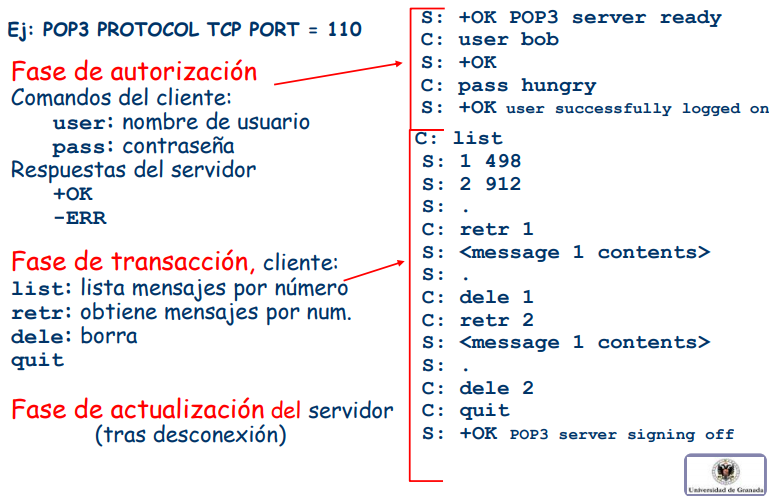
\includegraphics[scale=1,width=1\textwidth]{pop3.png}
\end{figure}

\textbf{IMAP4:} es un protocolo que permite trabajar con el correo como si fuese local. Un servidor IMAP asociará cada mensaje con una carpeta; cuando un mensaje llega al servidor, se asocia con la carpeta INBOX del destinatario, el cual puede entonces pasar el mensaje a una nueva carpeta creada por el usuario, leer el mensaje, borrarlo, etc. Este consta de 4 estados, \textbf{no autentiacado (NA)}, \textbf{autenticado (A)}, \textbf{seleccionado (S)} y \textbf{desconexión (D)}. \\

Comandos (puerto 143):
\begin{itemize}
\item CAPABILITY, NOOP, LOGOUT
\item NA $\rightarrow$ LOGIN, AUTHENTICATE
\item A $\rightarrow$ SELECT, CREATE, DELETE, LIST, APPEND, UN/SUBSCRIBE, \ldots
\item S $\rightarrow$ CHECK, CLOSE, SEARCH, FETCH, STORE, COPY, \ldots
\end{itemize}

\begin{verbatim}
#> telnet sal.ugr.es 143
* OK sal.ugr.es IMAP4rev1 v12.264 server ready
a001 LOGIN usuario clave
a001 OK LOGIN completed
a002 SELECT inbox
* 18 EXISTS
* 2 RECENT
* OK [UIDVALIDITY 3857529045] UID validity status
* OK [UIDNEXT 17] Predicted next UID
* FLAGS (\Answered \Flagged \Deleted \Draft \Seen)
* OK [PERMANENTFLAGS (\* \Answered \Flagged \Deleted \Draft \Seen)] Permanent flags
a002 OK [READ-WRITE] SELECT completed
a003 FETCH 12 full
* 12 FETCH (FLAGS (\Seen) INTERNALDATE "14-Jul-1993 02:44:25 -0700"
RFC822.SIZE 4282 ENVELOPE ("Wed, 14 Jul 1993 02:23:25 -0700 (PDT)"
"IMAP4 WG mtg summary and minutes"
(("Terry Gray" NIL "gray" "cac.washington.edu"))
((NIL NIL "imap" "cac.washington.edu"))
((NIL NIL "minutes" "CNRI.Reston.VA.US")
("John Klensin" NIL "KLENSIN" "INFOODS.MIT.EDU")) NIL NIL
"<B27397-0100000@cac.washington.edu>")
BODY ("TEXT" "PLAIN" ("CHARSET" "US-ASCII") NIL NIL "7BIT" 3028 92))
a003 OK FETCH completed
a004 FETCH 12 rfc822.header
* 12 FETCH (RFC822.HEADER {346}
Date: Wed, 14 Jul 1993 02:23:25 -0700 (PDT)
From: Terry Gray <gray@cac.washington.edu>
Subject: IMAP4 WG mtg summary and minutes
To: imap@cac.washington.edu
cc: minutes@CNRI.Reston.VA.US, John Klensin <KLENSIN@INFOODS.MIT.EDU>
Message-Id: <B27397-0100000@cac.washington.edu>
MIME-Version: 1.0
Content-Type: TEXT/PLAIN; CHARSET=US-ASCII
)
a004 OK FETCH completed
a005 STORE 12 +flags \deleted
* 12 FETCH (FLAGS (\Seen \Deleted))
a005 OK STORE completed
a006 LOGOUT
* BYE sal.ug.es IMAP4rev1 server terminating connection
a006 OK LOGOUT completed
#> _ 

\end{verbatim}

\begin{verbatim}
telnet capone.rutgers.edu 143
Trying 192.168.5.240...
Connected to 192.168.5.240.
Escape character is '^]'.
* OK [CAPABILITY IMAP4REV1 LOGIN-REFERRALS STARTTLS AUTH=LOGIN] capone.rutgers.edu
IMAP4rev1 2003.339 at Wed, 13 Apr 2005 01:38:58 -0400 (EDT)
Client A1 LOGIN mailtest Password
Server A1 OK [CAPABILITY IMAP4REV1 IDLE NAMESPACE MAILBOX-REFERRALS BINARY
UNSELECT SCAN SORT THREAD=REFERENCES THREAD=ORDEREDSUBJECT MULTIAPPEND]
User mailtest authenticated
Client A2 SELECT Inbox
* 2 EXISTS
* 2 RECENT
* OK [UIDVALIDITY 1113370837] UID validity status
* OK [UIDNEXT 3] Predicted next UID
* FLAGS (\Answered \Flagged \Deleted \Draft \Seen)
* OK [PERMANENTFLAGS (\* \Answered \Flagged \Deleted \Draft \Seen)]
Permanent flags
* OK [UNSEEN 1] first unseen message in /var/mail/mailtest
Server A2 OK [READ-WRITE] SELECT completed
Client A3 FETCH 2 BODY[HEADER]
* 2 FETCH (BODY[HEADER] {670}
Return-Path:
X-Original-To: mailtest@capone.rutgers.edu
Delivered-To: mailtest@capone.rutgers.edu
Received: from node18.rutgers.edu (node18 [192.168.5.38])
by capone.rutgers.edu (Postfix) with ESMTP id A291B2B15C
for ; Tue, 12 Apr 2005 22:23:53 -0400 (EDT)
Received: from me?here.com (unknown [192.168.5.250])
by node18.rutgers.edu (Postfix) with SMTP id 4653B14112
for ; Tue, 12 Apr 2005 22:24:03 -0400 (EDT)
To: some_guru@somewhere.com
From: pp@pp.com
Subject: Forged e-mail
Message-Id: <20050413022403.4653B14112@node18.rutgers.edu>
Date: Tue, 12 Apr 2005 22:24:03 -0400 (EDT)
)
* 2 FETCH (FLAGS (\Recent \Seen))
Server A3 OK FETCH completed
Client A4 FETCH 2 BODY[TEXT]
* 2 FETCH (BODY[TEXT] {88}
Hey,
The "To:" and "From:" are non-existent, but you still get the e-mail.
bye, bye
)
Server A4 OK FETCH completed
Client A5 LOGOUT
* BYE capone.rutgers.edu IMAP4rev1 server terminating connection
Server A5 OK LOGOUT completed
Connection closed by foreign host.
\end{verbatim}

\textbf{Correo electrónico Web.} Con este servicio, el agente de usuario es un navegador web corriente y el usuario se comunica con su buzón remoto a través de HTTP. Cuando un destinatario desea acceder a un mensaje de su buzón, este es enviado desde el servidor de correo del usuario al navegador del mismo utilizando el protocolo HTTP en lugar de los protocolos POP3 o IMAP. Cuando un emisor desea enviar un mensaje de correo electrónico, este es transmitido desde su navegador a su servidor de correo a través de HTTP en lugar de mediante SMTP. Sin embargo, el servidor de correo del emisor, continúa enviando mensajes a, y recibiendo mensajes de, otros servidores de correo que emplean SMTP. \\

\textbf{Ventajas IMAP4:} este protocolo que permite organizcaión en carpetas en el lado del servidor (MTA). Para ello, mantiene información entre sesiones asociando flagas a los mensajes. Permite la descarga de parte de los mensajes. Es posbile acceder con varios clientes, ahora bien POP también lo permite pero en modo descargar y guardar. \\

\textbf{Ventajas de Web MAIL:} en este se realiza la organización total en el servidor, que es accesible desde cualquier cliente con HTTP. En cuanto a la seguridad, una práctica extendida es el uso de HTTPS. \\

\textbf{Listado de puertos relacionados con e-mail:}

\begin{itemize}
\item POP3 - port 110
\item IMAP - port 143
\item SMTP - port 25
\item HTTP - port 80
\item Secure SMTP (SSMTP) - port 465
\item Secure IMAP (IMAP4-SSL) - port 585
\item IMAP4 over SSL(IMAPS) - port 993
\item Secure POP3 (SSL-POP) - port 995
\end{itemize}

En Linux se puede ver los servicios asociados a los puertos consultando el archivo 'etc/services'.

\section{Seguridad y protocolos seguros}
Para que una comunicación sea segura es deseable que cumpla las siguientes propiedades:

\begin{itemize}
\item \textit{Confidencialidad:} solo el emisor y el receptor deseado deberán comprender el contenido de los mensajes transmitidos. Puesto que los curiosos pueden interceptar los mensajes, es absolutamente necesario que los mensajes sean cifrados de alguna manera, de modo que un mensaje interceptado no pueda ser comprendido por el que lo ha interceptado. Este aspecto de la confidencialidad es probablemente el concepto más comunmente percibido del término comunicación segura.

\item \textit{Integridad de los mensajes:} dos usuarios que se comuniquen quieren estar seguros de que el contenido de sus comunicaciones no se ve alterado durante las transmisión ni maliciosamente ni por accidente.

\item \textit{Autenticación del punto terminal:} tanto el emisor como el receptor deberán poder confirmar la identidad del otro en el proceso de comunicación (confirmar que el otros es quien dice ser). Cuando las entidades se comunican a través de un medio en el que no es posible ver el otro, la autenticación no es tan sencilla.

\item \textit{Seguridad operacional:} casi todas las organizaciones actuales disponen de redes que están conectadas a la red pública Internet. Estas redes pueden, potencialmente, verse comprometidas. Los atacantes pueden intentar depositar gusanos en los hosts de la red, conseguir secretos corporativos, realizar un mapa de las configuraciones internas de la red y ejecutar ataques DoS. Para responder a los ataques efectuados contra la red de una organización se emplean dispositivos operacionales, como los cortafuegos y los sistemas de detección de intrusiones. Un cortafuegos se coloca entre la red de la organización y la red pública, controlando el acceso de paquetes procedentes de la red. Un sistema de detección de intrusiones realiza una 'inspección profunda de los pquetes', alertando a los administradores de la red cuando detecta cualquier actividad sospechosa.

\item \textit{No repudio o irrenunciablidad:} el sistema impide la renuncia de la autoría de una determinada acción.

\item \textit{Disponibilidad:} el sistema mantiene las prestaciones de los servicios con independencia de la demanda.
\end{itemize}
Se dice que una red de comunicaciones es 100\% segura si garantiza todos los aspectos que se acaban de ver. Ahora bien, no hay protocolos ni redes 100\% seguros. \\

La seguridad se debe situar en todos y cada uno de los niveles o capas, fijando el grado de seguridad el punto más débil. 

\textbf{Ataque de seguridad:} cualquier acción intencionada o nó que menoscaba cualquiera de los aspecto de seguridad. Dentro de la seguridad se presentan los siguientes tipos de ataque:

\begin{itemize}
\item \textbf{Sniffing:} vulneración a la confidencialidad, escuchas (husmear).

\item \textbf{Spoofing (phishing):} suplantación de la identidad de entidades.

\item \textbf{Man-in-the-middle:} hombre en medio (interceptación).

\item \textbf{Distributed Denial of Service (DDoS):} denegación de servicio distribuido, ejemplo Flooding (inundación).

\item \textbf{Malware:} troyanos, gusanos, spyware, backdoors, rootkits, ransomware, keyloggers,\ldots.
\end{itemize}

Veremos algunos tipos de cifrado:

\begin{itemize}
\item \textbf{Cifrado monoalfabético:}sustituya una letra del alfabeto por otra, ahora bien en lugar de hacerlo según un patrón, cualquier letra puede ser sustituida por cualquier otra siempre que cada una tenga una única letra y viceversa. A la hora de considerar lo fácir que puede ser a un atacante romper un cifrado monoalfabético podemos distinguir tres escenarios en función de la información que disponga el instruso:

	\begin{itemize}
	\item \textbf{Ataque de solo texto cifrado.} En alguno casos, el intruso puede tener acceso 		únicamente al texto cifrado interceptado, sin disponer de información segura acerca del 				contenido del mensaje en claro. Aunque la estadísitica ayuda a realizar ataques de solo cifrado. 	Por ejemplo, en español las vocales e y a son más comunes que las demás, además de que algunas 			combinaciones como as, es ,etc son bastante comunes, lo que ayuda descifrar el mensaje.

	\item \textbf{Ataque de texto en claro conocido.} Cuando un intruso conoce alguna de las parejas 	(texto en claro, texto cifrado) se dice que se trata de un ataque en claro conocido al esquema 		cifrado.

\item \textbf{Ataque de texto en claro seleccionado.} En un ataque de texto en claro seleccionado, el intruso tiene la posibilidad de elegir el mensaje de texto en claro y obtener su correspondiente texto cifrado.
	\end{itemize}

\item \textbf{Cifrado polialfabética:} permite mejorar el cifrado monoalfabético. La idea subyacente a este cifrado es utilizar varios cifrados monoalfabéticos, utilizando un cifrado monoalfabético específico para codificar cada letra situada en una posición específica dentro del mensaje de texto claro. De este modo, una misma letra que aparezca en diferentes posiciones dentro del mensaje en claso de podría codificar de forma distinta cada vez.

\item \textbf{Cifrados en bloque:} existen dos clases generales de técnicas de cifrado simétrico: los cifrados de flujo y los cifrados de bloque. En un cifrado de bloque, el mensaje que hay que cifrar se procesa en bloques de k bits. Por ejemplo, si k=64, entonces el mensaje se descompone en bloques de 64 bits y cada bloque se cifra de forma independientes. 

\item \textbf{Encadenamiento de bloques cifrados:} la idea básica sonsiste en enviar solo un valor aleatorio junto con el primer mensajes, y hacer que el emisor y el receptor utilicen los bloques codificados calculados, en lugar de los subsiguientes números aleatorios.
\end{itemize}

Vistos algunos ejemplo de ataques, se muestra mecanismos de seguridad:

\begin{itemize}
\item Cifrado (simétrico y asimétrico)
\item Autenticación con clave secreta (reto-respuesta)
\item Intercambio de Diffie-Hellman (establecimiento de clave secreta)
\item Funciones Hash. Hash Message Authentication Code (HMAC)
\item Firma Digital
\item Certificados Digitales
\end{itemize}

\textbf{Cifrado de datos:} es un procedimiento que sirve para garantizar la confidencialidad. Para ello se realiza la siguiente conversión, Texto llano/claro (P)$\rightarrow$ texto cifrado (C). Se basa en la existencia de un algoritmo de cifrado/descifrado, normalmente conocido $E_k()$ y $D_{k'}$. La dificultad reside en la existencia de una clave de cifrado $cifrado(k)/descifrado(k')$ desconocidas. 

\begin{figure}[h]
\centering
\caption{Esquema Cifrado de Datos}
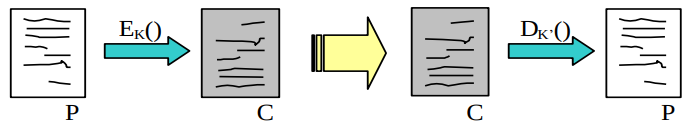
\includegraphics[scale=1,width=1\textwidth]{ejemplo_cifrado_datos.png}
\end{figure}

\textbf{Cifrado Simétrico, algoritmos de clave simétrica}: en este tipo de cifrado se usa una sola clave para cifrar y descifrar ($k=k'$). Entre los algoritmos de cifrado simétrico destacamos el \textbf{DES (\textit{'Data Encryption Standard'})}, que fue desarrollado por IBM en 1975. \\

El algoritmo DES toma una cadena de longitud fija de bits de texto plano y la transforma a través de una serie de complicadas operaciones en otro texto plano de igual longitud. En el caso del DES el tamaño del bloque son 64 bits. Además, por ser un algorimto de cifrado simétrico, DES utiliza una calve en la transformación, de forma que el desencriptado sólo lo pueden realizar aquellos que conocen la clave que se ha usado para encriptar. Esta clave es de 64 bit, aunque en la práctica sólo se usan 56, ya que 8 bits se usan solamenten para comprobar la paridad, y después se descartan. \\

El algoritmo DES lo que hace es coger una cadena de 64 bits, hacer un permutación inicial (otra al final, que invierte la permutación inicial) y dividirla en dos bloques de 32 bits. A uno de estos bloques le palica la función de Feistel y luego al resultado de esta se le aplica un XOR con el otro bloque de 32 bits. La función de Feistel o F-fucnión consiste en cuatro etapas (se muestran en la figura 22):

\begin{figure}[h]
\centering
\caption{Esquema DES}
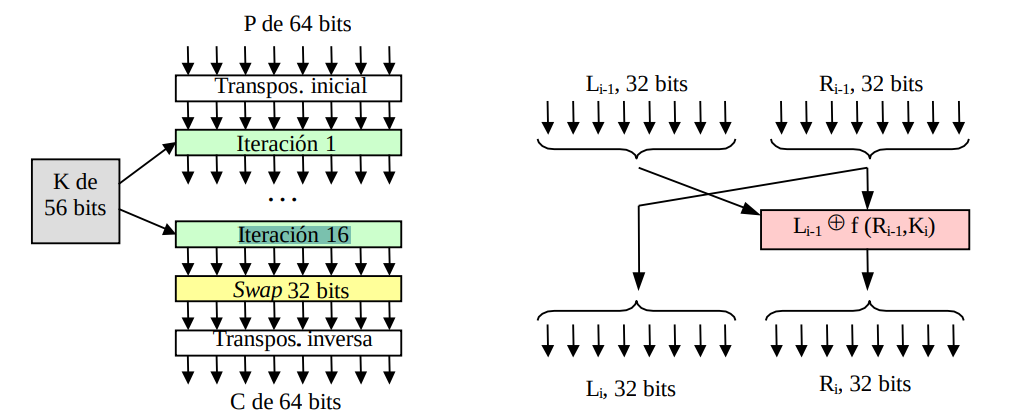
\includegraphics[scale=1,width=1\textwidth]{esquema_DES.png}
\end{figure}

\begin{itemize}
\item \textbf{Expansión:} el bloque de 32 bits se expande a 48 bits usando la expansión de permutación (E en la figura 22), duplicando así la mitdad de los bits. Las salida consiste en 8 piezas de 48-bits, cada una conteniendo una copia de 4 bits de entradas, más una copia del bit inmediatemente adyacente desde cada una de las pieces de salida.

\item \textbf{Mezclado de llave:} el resultado es combinado con una subclave usando una operación XOR. Dieciseis subclaves de 48-bits (una por pieza) se deriva de la clave principal. 

\item \textbf{Sustitución:} después de mezclar en la sublcave, el bloque es dividido en ocho piezas de 6-bits antes de procesarse en las cajas de sustitución o S-boxes. Cada una de las 8 cajas de sustitución reemplaza sus seis bits de entrada por 4 de salida de acuerdo a una transformación no lineal, provista en forma de 'lookup table'. Las cajas de sustitución proveen el núcleo de la seguridad del algoritmo DES.

\item \textbf{Permutation:} finalmente, las 32 salidas de las cajas de Sustitución se reorganizan conforme a una permutación fijada, P-box. Esto se diseña de forma que, tras permutar, los bits de salida de cada caja de sustitución en esta ronda se esparcen en la siguiente ronda en 4 cajas de sustitución diferentes.
\end{itemize}

\begin{figure}[h]
\centering
\caption{Esquema Función de Feistel}
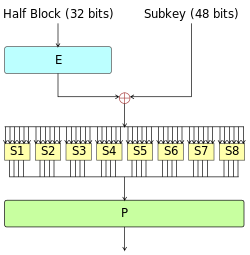
\includegraphics[scale=1,width=0.8\textwidth]{esquema_feistel.png}
\end{figure}

Como ya hemos visto el algoritmo DES es un esquema de cifrado de bloques. Encaminamiento DES (para evitar que DES sea un algorimto de sustitución):

\begin{figure}[h]
\centering
\caption{Ejemplo Encaminamiento DES}
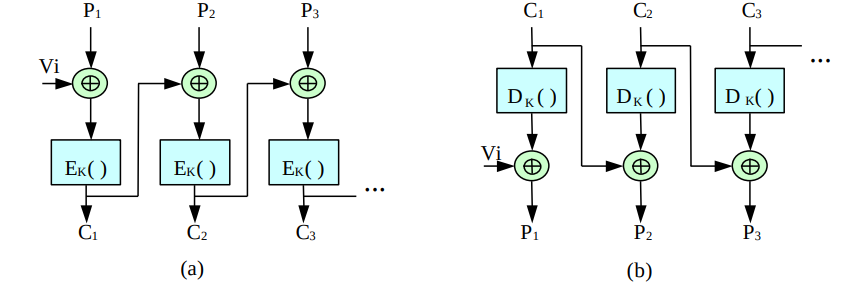
\includegraphics[scale=1,width=1\textwidth]{encaminamiento_des.png}
\end{figure}

Además, para mejorar la robuste surge el algoritmo DES doble y 3DES: \\

\begin{figure}[h]
\centering
\caption{Ejemplo DES doble y 3DES}
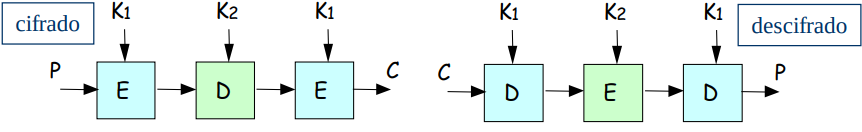
\includegraphics[scale=1,width=1\textwidth]{ejemplo_des_doble.png}
\end{figure} 

Otro algoritmo de encriptado simétrico es \textbf{IDEA ('\textit{International Data Encryption Algorithm'})}. Se trata de un algoritmo de cifrado simétrico, luego usa la misma clave para cifrar y descifrar. A diferencia del DES, las claves de IDEA tienen 128 bits y opera en tiempo real. \\

\begin{figure}[h]
\centering
\caption{Ejemplo IDEA}
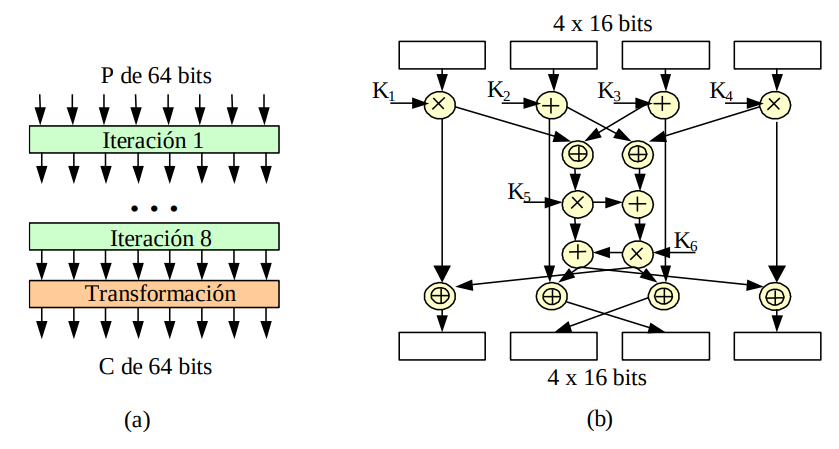
\includegraphics[scale=1,width=1\textwidth]{esquema_IDEA.png}
\end{figure}

\textbf{Cifrado asimétrico, algoritmos de clave pública/privada:} en esta caso se tiene dos claves por usuario (A), una clave pública $K_{pub_a}$ y otra privada $K_{pri_a}$ distintas. Si se conoce $K_{pub_a}$ es imposible conocer $K_{pri_a}$. De esta manera se usan claves diferentes para cifrar y descrifrar. \\

Cifrar: C=$E_{KpubB}(P)$ y Descifrar:$D_{KpriB}(C)$, es decir, se manda un mensaje cifrado con la clave pública y se descifra con la clave privada, que solo conoce el usuario dueño de dicha clave. Ahora bien si se manda un mensaje cifrado con la clave privada esto sirve como autenticación. \\

\textbf{RSA (Rivest, Shamir y Adleman):} en RSA existen dos componentes interrelacionados, la elección de las claves pública y privada y el algoritmo de cifrado y descifrado. Para genera las claves RSA pública y privada se lelvan a cabo los pasos siguientes:

\begin{enumerate}
\item El emisor elige dos números primos grandes, p y q. Cuanto maś grandes sean estos valores, más difícil será romper el algoritmos RSA, pero también se tardará maś en realizar la codificación y la decodificación. 

\item Calcula $n=p\cdot q$ y $z=(p-1)(q-1)$

\item Elige un número, $e$, menor que $n$, que no tiene ningún factor común (distinto de 1) con z (es decir, primo relativo). Se emplea la letra $e$ porque este valor se utilizará en el cifrado o encriptación.

\item Determina un número, $d$, tal que $ed-1$ es divisible de forma exacta por z. La letra $d$ se emplea porque este valor se utilizará en el descifrado. Dicho de otra manera, dado $e$, seleccionamos $d$ tal que:

\begin{equation*}
ed \> mod \> z=1
\end{equation*}

\item La clave pública que el emisor pone a disposición de todo el mundo, $K_B^+$, es la pareja de números $(n,e)$; su clave privada $K_B^-$, es la pareja de números $(n,d)$.
\end{enumerate}

El cifrado por parte del emisor y el cifrado por parte del emisor y el descifrado que lleva a cabo el receptor se hace de la siguiente manera: 

\begin{itemize}
\item Suponga que el emisor desea enviar al receptor un patrón de bits representado por el número entero m (con m < n). Para realizar la codificación, el emisor lleva a cabo la operación de exponenciación $m^e$, y luego calcula el resto entero que se obtiene al dividir $m^e$ entre n. En otras palabras, el valor cifrado, c, del mensaje de texto claro del emisor, m, es

\begin{equation*}
c = m^e \> mod \> n
\end{equation*}

El patrón de bits correspondiente a este texto cifrado c se envía al receptor.

\item Para descifrar el mensaje de texto cifrado recifido, c, el receptor hace el siguiente cálculo,

\begin{equation*}
m = c^d \> mod \> n
\end{equation*}
\end{itemize}

\begin{figure}[h]
\centering
\caption{Ejemplo RSA}
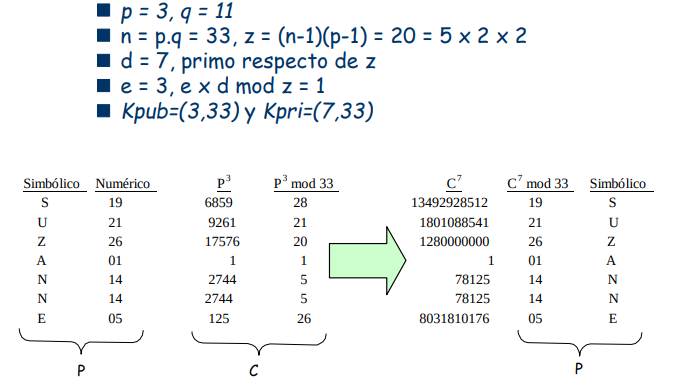
\includegraphics[scale=1,width=0.9\textwidth]{ejemplo_rsa.png}
\end{figure}

\textbf{Autenticación y cifrado de clave secreta:} 

\begin{figure}[h]
\centering
\caption{Esquema de reto-respuesta}
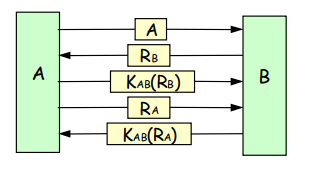
\includegraphics[scale=1,width=0.8\textwidth]{esquema_reto_respuesta.png}
\end{figure}

Los protocolos desafío-respuesta son una familia de protocolos que permiten la autenticación de entidades mediante el siguiente sistema:

\begin{enumerate}
\item Una parte (verificador) presenta una cestión (desafío).
\item La parte que se quiere autenticar recibe la cuestión y elabora una respuesta que envía al verificador.
\item El verificador recibe la respuesta  evalúa si la respuesta responde correctamente a la cuestión, y por tanto la entidad que envió la respuesta queda autenticada, o no.
\end{enumerate}

\textbf{Intercambio de Diffie-Hellman:} permite establecer una clave secreta entre dos entidades a través de un canal no seguro. Para dos partes A y B, que intentan establecer una clave secreta, y un adversario G, la versión básica es tal que:

\begin{itemize}
\item Se establece un primo \textbf{$n$} y un generador \textbf{$g\in \mathbb{Z}_p^*$}. Estos son públicos, conocidos no solo por las partes A y B sin otambién por el atacante G.

\item A escoge \textbf{$x\in Z_{n-1}$} al azar, calcula $A'=g^x \> mod \> n$, y lo envía a B.

\item B escoge \textbf{$y \in Z_{n-1}$} al azar, calcula $B'=g^y\> mod \> n$, y lo envía a A.
\end{itemize}
Nótese que tanto A' como B' pueden calcular $K=g^{x\cdot y} \> mod \> n$. Luego la clave compartida será K.

\begin{itemize}
\item A calcula $K_{AB}=(g^y \> mod \> n)^x$=$g^{yx} \> mod \> n$.
\item B calcula $K_{BA}=(g^x \> mod \> n)^y$=$g^{xy} \> mod \> n$.
\end{itemize}

\begin{figure}[h]
\centering
\caption{Esquema Diffie-Hellman}
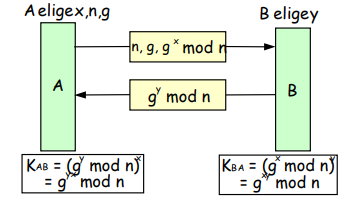
\includegraphics[scale=1,width=0.8\textwidth]{esquema_diffie_hellman.png}
\end{figure}

\textbf{Ataque man-in-the-middle:} se trata de un cyber-ataque donde el atacante secretamente retransmite y posiblemente altera las comunicaciones entre dos partes las cuales creen que se están comunicando directamente entre ellas.  \\

El intercambio Diffie-Hellman es sensible a ataques man-in-the-middle, pues si la comunicación es interceptada por un tercero (véase figura 30), éste se puede hacer pasar por el emisor de cara al destinatario y viceversa, ya que no se dispone de ningún mecanismo para validar la identidad de los participantes en la comunicación. Así, el man-in-the-middle podría acordar una clave con cada participante y retransmitir los datos entre ellos, escuchando la conversación en ambos sentidos.

\begin{figure}[h]
\centering
\caption{Esquema man-in-the-middle}
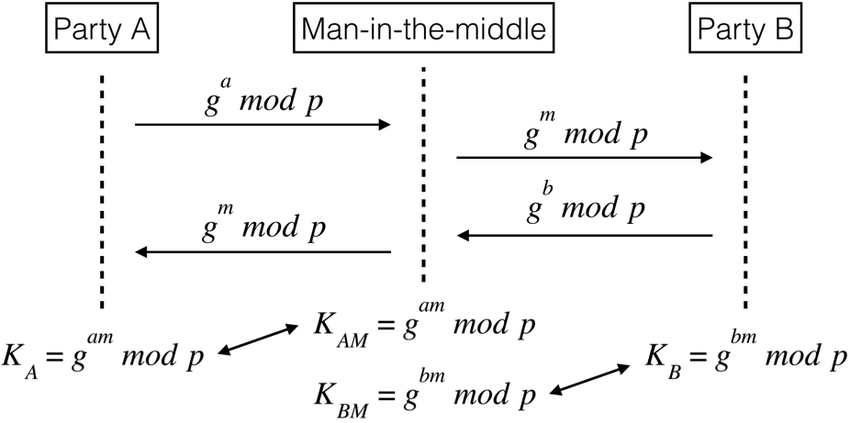
\includegraphics[scale=1,width=0.8\textwidth]{esquema_man-in-the-middle.png}
\end{figure}

\textbf{Funciones Hash (compendios):} 

\begin{itemize}
\item Funciones unidireccionales (irreversibles) de cálculo sencillo
\item Texto de entrada (M) de longitud variable
\item M $\rightarrow$ H(M) siendo H(M) de longitud fija (256 ó 512 bits)
\item Imposible obtener M a partir de su resumen H(M)
\item Invulnerables a ataques de colisión, dado M es imposible encontrar M' tal que $M \neq M'$ y $H(M)=H(M')$
\item Ejemplos de funciones HASH son MD5, SHA-1, SHA-512
\item Las funciones Hash se usan para garantizar integridad y autenticación. Para lo segundo utilizan Hash Message Authentication Code (HMAC):$M+H(K|M)$. Es más, para evitar ataques de extensión se usa $M+H(K|H(K|M))$
\end{itemize}

\textbf{MD5 ('Message Digest 5')}: este algoritmo calcula un valor hash de 128 bits mediante un proceso de cuatro pasos:

\begin{itemize}
\item Paso de relleno. Consiste en añadir un uno seguido del número de ceros suficiente para que la longitud del mensaje satisfaga ciertas condiciones, y con una longitud máxima de 448 bits.

\item Paso de agregación. Se añade una representación mediante 64 bits de la longitud del mensaje antes de la operación de relleno.

\item Inicialización MD buffer. Para calcular la función hash 'message-digest' se usa un buffer de cuatro palabras. Cada una de ellas es un registro de 32 bits. Estos registros se inicializan usando los siguiente valores en hexadcimal, con los bytes de menor orden primero:

\begin{verbatim}
word A: 01 23 45 67
word B: 89 ab cd ef
word C: fe dc ba 98
word D: 76 54 32 10
\end{verbatim}

\item Bucle final en el que se procesan los bloques de 16 palabras del mensaje (512 bits). Primero definimos cuatro funciones auxiliares donde cada una toma como entrada tres palabras de 32 bits y produce como salida una palabra de 32 bits.

\begin{verbatim}
F(X,Y,Z) = XY v not(X) Z
G(X,Y,Z) = XZ v Y not(Z)
H(X,Y,Z) = X xor Y xor Z
I(X,Y,Z) = Y xor (X v not(Z))
\end{verbatim}

\end{itemize}

\begin{figure}  +
\centering
\caption{Ejemplo Algoritmo MD5}
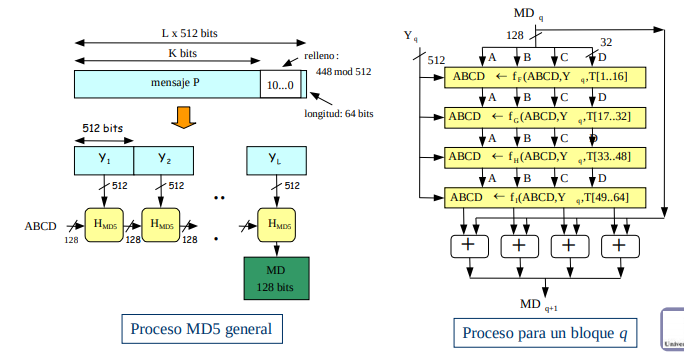
\includegraphics[scale=1,width=0.9\textwidth]{ejemplo_md5.png}
\end{figure}

\textbf{SHA-1(\textit{'Secure Hash Algorithm 1'}, NIST 1993):} este algoritmo está basado en una serire de principios similares a los utilizados en el diseño de MD4, el predecesor de MD5. SHA-1, un estándar federal del gobierno de EEUU, es obligatorio siempre que se requiera un algoritmo hash criptográfico apra aplicaciones gubernamentales. Este algoritmo produce un resument del mensaje (\textit{message digest)} de 160 bits. Esa mayor longitud de salida hace que SHA-1 sea más seguro. \\

\textbf{Ataques contra SHA-1:} en el año 2005 la resistencia de esta algoritmo se vió comprometida como consecuencia de que en el año 2004 el algoritmo MD5 quedase comprometido. Un equipo de investigación chino demostró que es capaz de romper el algoritmo SHA-1 en al menos $2^69$, que si bien sigue siendo un número muy grande está dentro de las capacidades de computación actuales. \\

En la figura 31 se observa que el algoritmo SHA-1 es similar al MD5, con la diferencia de que la salida es una cadena de 160 bits en lugar de 128 lo que lo hace más seguro como ya se había predicho.

\begin{figure}[h]
\centering
\caption{Esquema SHA-1}
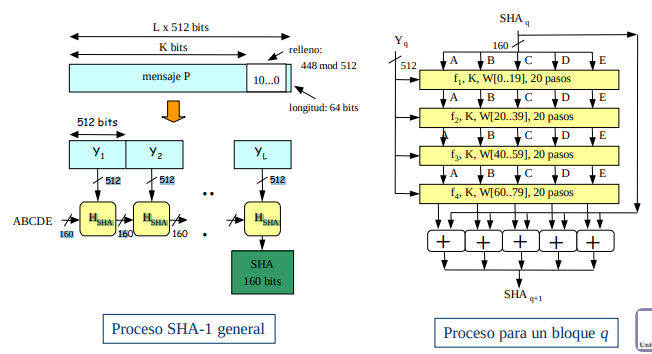
\includegraphics[scale=1, width=0.9\textwidth]{esquema_sha-1.png}
\end{figure}

\textbf{Firma digital:} es una técnica criptográfica que permite,

\begin{itemize}
\item Que el receptor pueda autenticar al emisor.
\item Que no haya repudio
\item Que el emisor tenga garantías de no falsificación (integridad)
\end{itemize}

\textbf{Firma digital con clave secreta: Big Brother.} Esta firma digital usa una clave secreta simétrica. \\

\begin{figure}[h]
\centering
\caption{Esquema firma digital con clave secreta ('Big Brother')}
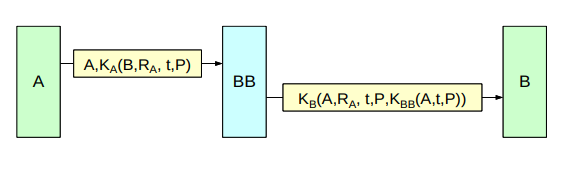
\includegraphics[scale=1,width=0.8\textwidth]{firma_big_brother.png}
\end{figure}

\textbf{Firma digital con clave asimétrica. Doble cifrado:}

\begin{itemize}
\item Un cifrado para propocionar privacidad, con $K_{pubB}$
\item Otro cifrado para proporcionar autenticación $K_{priA}$
\item Para firma, se envia $K_{pubB}(K_{priA}(T))$
\item En el receptor $K_{pubA}(K_{priB}(K_{pubB}(K_{priA}(T))))=T$
\end{itemize}

\textbf{Debilidad:} para garantizar el no repudio se necesita garantizar la asociación fehaciente e indisoluble de la 'identidad A' con su 'clave pública $K_{pubA}$', esto se consigue con un 'certificado digital'. \\

Como ya se ha dicho para garantizar la asocicación 'identidad-clave' se utilizan los certificados digitales. \\

\textbf{Autoridades de certificación (AC):} son entidades para garantizar la asociación entre identidad y claves.

\begin{itemize}
\item El usuario obtiene sus claves pública y privada.
\item Este envía una solicitud, firmada digitalmente a la AC, indicando su identidad y su clave pública.
\item AC comprueba la firma y emite el certificado solicitado:
	\begin{itemize}
		\item Identidad de AC, identidad del usuario, clave pública del usuario y otros datos como, por ejemplo, el período de validez del certificado.
		\item Todo ello se firma digitalmente con la clave privada de AC con objeto de que el certificado no pueda falsificarse.
	\end{itemize}
\end{itemize}

El formato de certificados es principalmente X.509. Este es un estándar UIT-T (UTHH Sector de Normalización de las Telecomunicaciones de la UIT), que especifica, entre otras cosas, formatos estándar para certificados de claves públicas y un algoritmo de validación de la ruta de certificación. Su sintaxis, se define empleando el lenguaje ASN.1, y los formatos de codificación maś comunes son DER (\textit{Distinguish Encoding Rules)} o PEM (\textit{Privacy Enhanced Mail}). \\

Entreo las autoridades de certificación reconocidas se tiene:

\begin{itemize}
\item ACE (\url{ww.ace.es})
\item CAMERFIRMA (\url{www.camerfirma.es})
\item CERES (\url{www.cert.fnmt.es})
\item VeriSign (\url{www.verisign.com})
\end{itemize}


Campos de un certificado digital X.509:

\begin{tabular}{|l|l|}
\hline
Campo & Explicación \\
\hline
Versión & Número de versión de la especificación X.509 \\
\\\hline
Número de Serie & El único identificador usado por la AC \\
\hline
Firma & Firma del certificado \\
\hline
Editor & Nombre de la AC definida por X.509 \\
\hline
Periodo Validez & Inicial y final del periodo de validez del certificado \\
\hline
Nombre entidad & La entidad cuya clave pública se certifica \\
\hline
InforLlave pública & La clave pública de la entidad y los algoritmos que usa \\
\hline
\end{tabular}
\\

\begin{verbatim}
Certificate:
Data:
Version: 1 (0x0)
Serial Number: 7829 (0x1e95)
Signature Algorithm: md5WithRSAEncryption
Issuer: C=ZA, ST=Western Cape, L=Cape Town, O=Thawte Consulting cc,
OU=Certification Services Division,
CN=Thawte Server CA/Email=server-certs@thawte.com
Validity
Not Before: Jul 9 16:04:02 1998 GMT
Not After : Jul 9 16:04:02 1999 GMT
Subject: C=US, ST=Maryland, L=Pasadena, O=Brent Baccala,
OU=FreeSoft, CN=www.freesoft.org/Email=baccala@freesoft.org
Subject Public Key Info:
Public Key Algorithm: rsaEncryption
RSA Public Key: (1024 bit)
Modulus (1024 bit):
00:b4:31:98:0a:c4:bc:62:c1:88:aa:dc:b0:c8:bb:
33:35:19:d5:0c:64:b9:3d:41:b2:96:fc:f3:31:e1:
66:36:d0:8e:56:12:44:ba:75:eb:e8:1c:9c:5b:66:
70:33:52:14:c9:ec:4f:91:51:70:39:de:53:85:17:
16:94:6e:ee:f4:d5:6f:d5:ca:b3:47:5e:1b:0c:7b:
c5:cc:2b:6b:c1:90:c3:16:31:0d:bf:7a:c7:47:77:
8f:a0:21:c7:4c:d0:16:65:00:c1:0f:d7:b8:80:e3:
d2:75:6b:c1:ea:9e:5c:5c:ea:7d:c1:a1:10:bc:b8:
e8:35:1c:9e:27:52:7e:41:8f
Exponent: 65537 (0x10001)
Signature Algorithm: md5WithRSAEncryption
93:5f:8f:5f:c5:af:bf:0a:ab:a5:6d:fb:24:5f:b6:59:5d:9d:
92:2e:4a:1b:8b:ac:7d:99:17:5d:cd:19:f6:ad:ef:63:2f:92:
ab:2f:4b:cf:0a:13:90:ee:2c:0e:43:03:be:f6:ea:8e:9c:67:
d0:a2:40:03:f7:ef:6a:15:09:79:a9:46:ed:b7:16:1b:41:72:
0d:19:aa:ad:dd:9a:df:ab:97:50:65:f5:5e:85:a6:ef:19:d1:
5a:de:9d:ea:63:cd:cb:cc:6d:5d:01:85:b5:6d:c8:f3:d9:f7:
8f:0e:fc:ba:1f:34:e9:96:6e:6c:cf:f2:ef:9b:bf:de:b5:22:
68:9f
\end{verbatim}

\textbf{Protocolos Seguros}.

\begin{itemize}
\item \textbf{Seguridad Perimetral.} Hay dos tipos de herramientas seguras en una red, por un lado tenemos las seguridad peritmetral que sirve para regular el acceso de usuarios, comunicaciones, etc. a los usuarios de una red y por otro lado, las comunicaciones seguras. \\

La seguridad digital son los firewall, los sistemas de detección de intrusiones (IDS) y de respuesta (IRS) que permiten tomar una respuesta a determinados ataques.

\item \textbf{Seguridad (criptográfica) en protocolos.} Se definen en las distintas capas que tenemos definidas en TCP/IP. Tenemos distintos tipos de protocolos dependiendo de la capa en la que se encuentren. Proveer de un protocolo seguro en capa de aplicación es menos seguro que proveer de un protocolo seguro en capa de enlace, ya que un protocolo de aplicación sólo encripta el payload mientras que una de capa enlada encripta todo menos la capa de enlace.
	\begin{itemize}
		\item \textbf{Capa de aplicación}
			\begin{itemize}
				\item Pretty Good Privacy (PGP)
				\item Secure Shell (SSH)
			\end{itemize}
		\item \textbf{Capa de sesión (entre aplicación y transporte)}
			\begin{itemize}
				\item Transport Secure Layer (TSL) (sucesor de SSL) $\rightarrow$ HTTPS, IMAPS, SSL-POP, VPN. \\
				TLS= Handshake (negociar) + Record Protocol (operación). (mirar glosario) \\
				TLS $\rightarrow$ confidencialidad ($K_{secreta}$ negociada + Autenticación (para el server por defecto con $K_{publica}$ + integriadad (con HMAC)
			\end{itemize}
		\item \textbf{Capa de red} $\rightarrow$ IPSec(VPN)
	\end{itemize}
\end{itemize}

\section{Aplicaciones multimedia}
IP es una tecnología de convergencia, lo cual implica que permite el uso de aplicaciones multimeda (audio, video, juegos, real-time). Ya hemos hablado del término Calidad de servicio (QoS), que es la capacidad de ofrecer el rendimiento requerido para una aplicación. IP ofrece su mejor esfuerzo, sin embargo, no garantiza la calidad de servicio. \\

\textbf{Tipos de aplicaciones:}

\begin{itemize}
\item Flujo de audio y vídeo (streaming) almacenado $\rightarrow$ Ej. Youtube.
\item Flujo de audio y vídeo en vivo $\rightarrow$ Ej. emisoras de radio o IPTV
\item Audio y vídeo interactivo $\rightarrow$ Ej. Skype
\end{itemize}

\textbf{Característica fundamentales:}

\begin{itemize}
\item Elevado ancho de banda.
\item Tolerantes relativamente a la pérdida de datos. Si se pierde algún paquete en la transferencia de datos no se produce ningún error catastrófico, es más probablemente el usuario ni se de cuenta.
\item Exigen Delay (retardo) acotado. Si el delay no estuviera acotado significa que se podría dar el caso en el que los paquete tardasen demasiado en llegar al usuario, de forma que notaría cortes en el video.
\item Exigen Jitter (fluctuación del retardo) acotado. El jitter es la variación del delay. Un video necesita un delay lo más constante posible. Si tenemos un delay constante de un segundo, se puede administrar correctamente el espacio del buffer. En cambio si hay un cambio de delay muy brusco el video se verá entrecortado
\item Se pueden beneficiar de usar multicast (direcciones destino de grupo). Básicamente lo que permite es reducir el ancho de banda ocupado por las aplicaciones multimedia. Si varios usuarios piden un mismo archivo, el servidor, en vez de mandar una respuesta unicast para cada petición manda una respuesta multicast para todos, de forma que el archivo es mandado una única vez.
\end{itemize}

\begin{figure}[h]
\centering
\caption{Esquema Router con QoS}
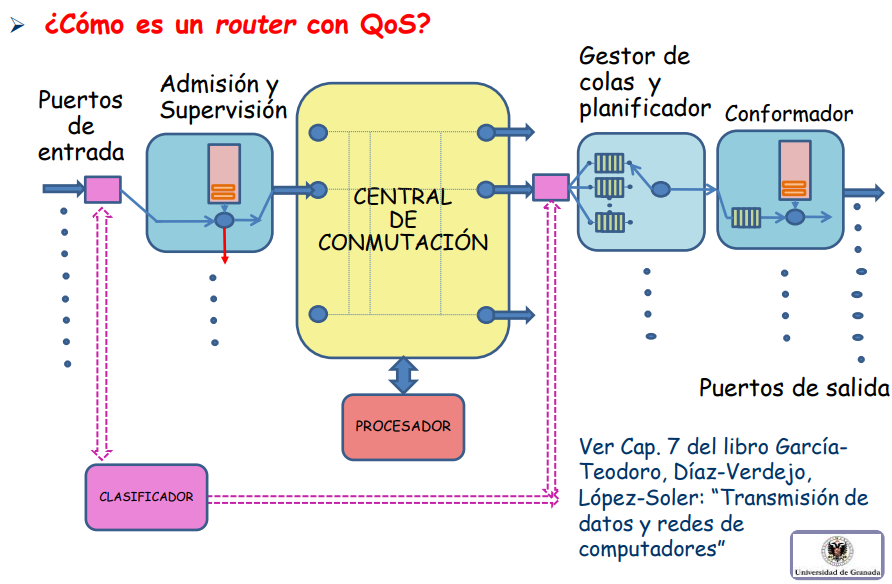
\includegraphics[scale=1,width=0.8\textwidth]{router_qos.png}
\end{figure}

\section{Aplicaciones para interconectividad de redes locales}
\textbf{DHCP (Dynamic Host Configuration Protocol:} se trata de un protocolo que provee un marco de trabajo para pasar información de configuración a los terminales en una red TCP/IP. Concretamente, DHCP proporciona parametros de configuración a los host de Internet. Este se compone de un protocolo para entregar parámetros de configuración específica de cada host desde un servidor DHCP y un mecanismo para reservar direcciones red para los hosts.´  DHCP está basado en el protocolo Bootstrap (BOOTP), añadiendole las opciones de configuración adicional. DHCP captura el comportamiento de agentes de retraso BOOTP, y los participantes DHCP pueden interoperar con participantes BOOTP. \\

El protocolo DHCP, como ya hemos dicho es un protocolo UDP y opera sobre el puerto 67.

\begin{itemize}
\item El host (cliente) envía un mensaje broadcast: 'DHCP discover'
\item El server DHCP responde con un mensaje: 'DHCP offer'.
\item El host solicita una dirección IP, mensaje 'DHCP request'
\item El server DHCP envía la dirección IP: mensaje 'DHCP ack'
\end{itemize}

Ahora se explicarán brevemente las funciones y significados de cada uno de los mensajes DHCP del cliente.

\begin{itemize}
\item \textbf{DHCPDISCOVER.} Cuando un servidor recibe este mensaje de un cliente, el servidor elige una dirección de red para el cliente solicitante. Si no hay direcciones disponibles, el servidor puede elegir reportar el problema al administrador del sistema. Si una dirección está disponible, la nueva dirección se selecciona.

\item \textbf{DHCPREQUEST.} Un mensaje de este tipo puede venir de un cliente respondiendo a un mensaje DHCPOFFER del servidor, de un cliente verificando una dirección IP reservada previamente o de un cliente extendiendo la ocupación de una dirección de red. 

\item \textbf{DHCPRELEASE.} Tras recibir un mensaje de este tipo, el servidor marca la dirección red como no reservada. El servidor debería retener un registro de los parámetros de inicialización del cliente para posible reutilización en respuesta a petciones siguientes del cliente.
\end{itemize}

\begin{figure}[h]
\centering
\caption{Esquema DHCP}
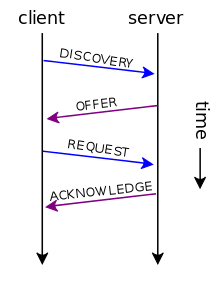
\includegraphics[scale=1,width=0.6\textwidth]{esquema_dhcp.png}
\end{figure}

\section{Glosario}
\begin{itemize}
\item \textbf{Suite de Internet:} conjunto de aplicaciones relacionadas con internet (navegador web, cliente de correo electrónico, ...)

\item \textbf{Paquetes Conmutados:} grupos de información que consta de dos partes (los datos propiamente dichos y la información de control, que indica la ruta a seguir a lo largo de la red hasta el destino del paquete) y que han sido transmitidos por conmutación de paquetes, es decir, se han agrupado los datos transmitidos a través de una red digital de paquetes. 

\item \textbf{Socket:} descriptor de una transmisión a través del cual la aplicación puede enviar y/o recibir información hacio y/o desde otro proceso de aplicación. Es una 'puerta' de acceso entre la aplicación y los servicios de transporte.

\item \textbf{Teoría de colas:} estudio de las líneas de espera que se producen cuando llegan clientes demandando un servicio, esperando si no se les puede atender inmediatamente y partiendo cuando ya han sido servidos.

\item \textbf{Modelo M/M/1:} Las colas poissonianas (o exponenciales o markovianas) son modelos tipo M/M, con llegadas de Poisson y servicio exponencial. El modelo M/M/1 dispone sólo de un canal para dar servicio, las llegadas siguen un proceso de Poisson y la distribución del tiempo de servicio es exponencial.

\item \textbf{TLV (Type-Length-Value):} es un formato de representar información, de forma que haya información que pueda tener presencia opcional y longitud variable.

\item \textbf{SOA (Start of Authority):} es un tipo de registro en el DNS que contiene información administativa sobre la zona de la que es autoridad,  espcialmente fijándose en las zonas de transferencias.

\item \textbf{Resource Record (RR):} es la unidad de información inicial en los archivos de zona DNS. Los RR son los bloques de construcción básicos de host-name y información IP y se usan para resolver todas las consultas DNS.

\item \textbf{Cookie:} es un término que hace referencia a una pequeña información enviada por un sitio web y almacenada en el navegador del usuario, de manera que el sitio web puede consultar la actividad previa del navegador. Si se ha realizado un curso desde un inicio o una nueva aplicación se pueden realizar con la misma contraseña o no en su sistema.

\item \textbf{URI (identificador de recursos uniforme):} es una cadena de caracteres que identifica los recursos de una red de forma unívoca. La diferencia respecto a un localizador de recursos uniforme (URL) es que estos últimos hacen referencia a recursos que, de forma general, pueden variar en el tiempo.

\item \textbf{MIME (Multipurpose Internet Mail Extension}: STD 11, RFC 822, define un protocolo de representación de mensajes detallando bastante las cabeceras de mensajes US-ASCII, y deja el contenido de mensaje, o cuerpo del mensaje, como texto plano US-ASCII. Este conjunto de documentos, colectivamente llamados MIME, redefine el formato de mensajes que se permiten para
	\begin{itemize}
		\item Cuerpos de mensajes textuales en conjuntos de caracteres distintos a US-ASCII
		\item Un conjunto extensible de diferentes formatos para cuerpos de mensajes no textuales
		\item Cuerpos de mensajes multiparte
		\item  Información textual de la cabecera en conjuntos de caracteres distintos a US-ASCII.
	\end{itemize}

\item \textbf{SYN:} es un bit de control del segmento TCP, que se utiliza par sincronizar los número de secuencia inciales de una conexión en el procedimiento de establecimiento de tres fases (3 way handshake). Se usa para sincronizar los números de secuencia en tres tipos de segmentos, petición de conexión, confimación de conexión (con ACK activo) y recepción de la confirmación (con ACK activo).	  

\item \textbf{Ataque por repetición:} es un tipo de ataque en el cual el atacante captura la información que viaja por la red, por ejemplo un comando de autenticación que se envía a un sistema informático, para, posteriormente, enviarla de nuevo a su destinatario, sin que este note que ha sido capturada. Si el sistema informaico o aplicación es vulnerable a este tipo de ataques, el sistema ejecutará el comando, como si fuera legítimo, enviando la respuesta al atacante que puede así obtener acceso al sistema.

\item \textbf{Flooding DDoS Attack:} los ataques de este tipo utilizan lo que parecen ser peticiones legitimas para atacar una aplicación o servidor. Estos ataques a menudo se basan e un 'botnet', que es un grupo de ordenadores conectados por internet que han sido apropiados maliciosamente a través del uso de malware.

\item \textbf{Ataque de Reflexión:} se trata de un tipo de ataque DDoS que utiliza una nueva herramienta de red llamada memcached. Los ataques de reflexión utilizan tráfico UDP falso desde un servidor que aloja el servicio explotado para forzar el envío de datos a una víctima desprevenida.

\item \textbf{Memcached:} es un sistema distribuido de propósito general para caché basado en memoria. Este es empleado para el almacenamiento en caché de datos u objetos en la memoria RAM, reduciendo así las necesidades de acceso a un origen de datos externo.

\item \textbf{Sistema de detección de intrusiones (IDS):} es un programa de detección de accesos no autorizados a un computador o a una red. El IDS suele tener sensores virtuales (por ejemplo, un 'sniffer' de red) con los que el núcleo del IDS puede obtener datos externos. El IDS detecta, gracias a dichos sensores, las anomalías que pueden ser indicio de la presencia de ataques y falsas alarmas. No bloquean el tráfico, sino que lo analizan en busca de anomalías. Si además ofrece una respuesta para una anomalía entonces es un sistema de respuesta a intrusiones (IRS).

\item \textbf{Sistema de prevención de instrusos (IPS):} es un software que ejerce el control de acceso en una red informática para proteger a los sistemas computacionales de ataques y abusos. La tecnología de prevención de intrusos es considerada por algunos como una extensión de los sistemas de detección de intrusos (IDS), pero en realidad es otro tipo de control de acceso, más cercano a las tecnologías cortafuegos.

\item \textbf{Pretty Good Privacy (PGP):} es un esquema general de seguridad que originalmente se diseñó orientado al coreo electrónico pero es casi un mecanimso genérico. Incorpora criptografía simétrica para confidencialidad, criptografía asimétrica para intercambio de claves, firma electrónica y certificado, aunque los certificados PGP no siguen la filosofía de los certificados emitidos por una AC, siguen la misma idea.

\item \textbf{Secure Shell (SSH):} es el nombre de un protocolo y programa que lo implementa cuya principal función es el acceso a un servidor por medio de un canal seguro en el que toda la información está cifrada. Además de la conexión a otros dispositivos, SSH permite copiar datos de forma segura, gestionar claves RSA para no escribir contraseñas al conectar los dispositivos y pasar los datos de cualquier otra aplicación por un canal seguro tunelizado mediante SSH y también puede redirigir el traico del Sistema de Ventanas para poder ejecutar programas gráficos remotamente.

\item \textbf{Transport Layer Security (TLS):} es un protocolo cuyo principal objetivo es proveer privacidad e integridad entre dos aplicaciones que se comuniquen. Este se compone de dos capas, el TLS Record Protocol y el TLS Handshake Protocol. TLS tiene dos propiedades básicas, la primera es que la conexión  es privada, y lo segundo que es fiable. Es además una mejora respecto al sistema SSL.

\item \textbf{Secure Sockets Layer (SSL)}: SSL se emplea a menuda para proporcionar seguridad a las transacciones que tienen lugar a través de HTTP. Sin embargo, puesto que SSL dota se seguridad a TCP, puede ser empleado por cualquier aplicación que se ejecute sobre TCP. SSL proporciona una API simple con sockets, que es similar y análoga a la API de TCP.

\item \textbf{IPSec:} se utiliza para conexiones VPN. IPSec, al trabajar en capa de red, encripta toda la comunicación incluida la capa de red del dispositivo porque lo que hace es un túnel donde encripta toda esta parte (de capa de red hacia arriba) y lo mete en otro paquete de capa de red.Funciona muy bien porque el paquete no necesita ser desencriptado en el siguiente paso sino que se desencripta al llegar al destino. Por eso podemos hacer una VPN con IPSec.

\item \textbf{Boot strap Protocol (BOOTP):} es un protocolo de red UDP utilizado por los clientes de red para obtener su dirección IP automáticamente.

\item \textbf{Dirección IP:} magnitud de 32 bits que identifica de forma únivoca a un host.

\item \textbf{Mnemóncio:} es una palabra que sustituye a un código de operación, con lo cual resulta más fácil la programación, es de aquí de donde se aplica el concepto de lenguaje ensamblador.
\end{itemize}


\section{Bibliografía}
\begin{enumerate}
\item \href{https://tools.ietf.org/html/rfc2045#page-5}{RFC 2045}
\item \href{https://tools.ietf.org/html/rfc2109}{RFC 2109}
\item \href{https://tools.ietf.org/html/rfc6838}{RFC 6838}
\item \href{https://tools.ietf.org/html/rfc1521#page-9}{RFC 1521}
\item \href{https://tools.ietf.org/html/rfc1321}{RFC 1321}
\item \href{https://tools.ietf.org/html/rfc2131#section-4.3}{RFC 2131}
\item \href{https://tools.ietf.org/html/rfc1034}{RFC 1034}
\item \href{https://tools.ietf.org/html/rfc1035}{RFC 1035}
\item \href{https://tools.ietf.org/html/rfc6265#section-5.2}{RFC 6265}
\item \href{https://developer.mozilla.org/es/docs/Web/HTTP/Headers}{Developer Mozila, Headers}
\item James F.Kurose, Keith W.Ross, 'Redes de computadores. Un enfoque descendente', 7ª edición, Ed.Pearson.
\item {Juan M.Lopez Soler y Jorge Navarro Ortiz, 'Apuntes Fundamentos de Redes'}

\end{enumerate}

\end{document}